\documentclass[aspectratio=169]{beamer}
\usepackage[alf,abnt-etal-cite=3,abnt-etal-list=3,abnt-url-package=url,abnt-emphasize=bf,abnt-etal-text=emph]{abntex2cite}
\usepackage{caption}            % remodelando o formato dos títulos de 
\usepackage{subfigure}           % figuras dentro de figuras
\usepackage{tikz}
\usepackage[T1]{fontenc}         % usa fontes postscript com acentos
\usepackage[brazil]{babel}       % hifenização e títulos em português do Brasil
\usepackage[utf8]{inputenc}     % permite edição direta com acentos
\usepackage{amsmath}             % pacote da AMS para Matemática Avançada
\usepackage{amssymb}             % símbolos extras da AMS
\usepackage{latexsym}            % símbolos extras do LaTeX
\usepackage{graphicx}            % para inserção de gráficos
\usepackage{listings}            % para inserção de código
\usepackage{fancyvrb}            % para inserção de saídas de comandos

\newcommand{\backgroundlogo}{
  \begin{tikzpicture}[remember picture,overlay]
    \node[opacity=0.1,anchor=center] at (current page.center) {%
      
\includegraphics[width=10cm]{logoufla.jpg}
    };
  \end{tikzpicture}
}
\captionsetup[figure]{labelformat=empty}% redefines the caption setup of the figures environment in the beamer class.

\graphicspath{{./images}}

\usetheme{default}

\definecolor{UFLAblue}{HTML}{224271}

\definecolor{UFLAgreen}{HTML}{00793c}

\setbeamercolor{title}{fg=UFLAblue}
\setbeamercolor{frametitle}{fg=UFLAblue}

\setbeamercolor{titlelike}{fg=UFLAblue}
\setbeamercolor{section in toc}{fg=UFLAblue}

\setbeamercolor{caption name}{fg=black}

\setbeamercolor{secondary}{fg=black}

\setbeamercolor{normal text}{fg=black}

\setbeamertemplate{section page}
{
    \begin{centering}
    \begin{beamercolorbox}[sep=12pt,center]{part title}
    \usebeamerfont{section title}\insertsection\par
    \end{beamercolorbox}
    \end{centering}
}

\AtBeginSection{\frame{\sectionpage}}

\title[Presente Trabalho]{\textbf{CONTROLE DE TRAJETÓRIA DE IMPRESSORAS 3D UTILIZANDO ALGORITMO ITERATIVO E PROGRAMAÇÃO NÃO LINEAR}
}
\author[Joao]{João Vivas Cisalpino}

\institute[UFLA]{Orientador: Wander Gustavo Rocha Vieira \\ Universidade Federal de Lavras}

\date{08/12/2023} % Data da apresentação

\begin{document}

\begin{frame}
  \backgroundlogo
  \titlepage
\end{frame}

\logo{
\includegraphics[width=2cm]{logoufla.jpg}}

\begin{frame}
  \frametitle{Sumário}
  \setcounter{tocdepth}{1}
  \tableofcontents
  % Conteúdo do slide aqui
\end{frame}

\section{\insertsectionnumber . Introdução}

\begin{frame}
  \frametitle{\insertsection}
  Manufatura aditiva
  \begin{itemize}
    \item Alta iterabilidade
    \item Produção em pequena escala
    \item Reprodutibilidade
    \item Facilidade de lidar com geometrias complexas
  \end{itemize}
  
  \textit{Fused Deposition Modeling} (FDM):
    \begin{itemize}
      \item Acessibilidade crescente.
      \item Aplicabilidade em diversas áreas como no setor automobilístico.
    \end{itemize}

  Tempo de impressão como principal limitação:
    \begin{itemize}
      \item Restringe a aplicabilidade para peças maiores.
      \item Limita a aplicabilidade como planta produtiva.
    \end{itemize}
\end{frame}


\subsection{\insertsectionnumber .\insertsubsectionnumber . Objetivos}
\begin{frame}
  \frametitle{\insertsubsection}
  Objetivo geral:
  \begin{itemize}
    \item Investigar e desenvolver uma metodologia para atuação de controle de trajetória em impressoras 3D FDM de forma a possibilitar maiores velocidades e garantindo a precisão dimensional das peças produzidas.
  \end{itemize}
  Objetivos específicos:
  \begin{itemize}
    \item Desenvolver um algoritmo iterativo que possa ser integrado ao sistema de controle de impressoras 3D para minimizar os desvios entre o percurso desejado e o efetivamente percorrido, levando em consideração a dinâmica da impressora.
    \item Simular o comportamento da impressora 3D com o novo algoritmo para avaliar o comportamento do método em relação aos parâmetros controlados.
  \end{itemize}

\end{frame}

\section{\insertsectionnumber . Referencial Teórico}

\subsection{\insertsectionnumber .\insertsubsectionnumber . Manufatura Aditiva}
\begin{frame}
  \frametitle{\insertsubsection}
  Definido por:
  \begin{itemize}
    \item Construir o modelo de forma aditiva, como implica o nome.
    \item Dispensar a necessidade de planejar as operações de maneira individual para fabricar um modelo tridimensional.
  \end{itemize}
  Pode utilizar diversos processos como:
  \begin{itemize}
    \item Extrusão (fusão e solidificação)
    \item Sinterização a laser (aglutinação)
    \item Estereolitografia (cura por luz)
  \end{itemize}
\end{frame}

\subsection{\insertsectionnumber .\insertsubsectionnumber . \textit{Fused Deposition Modeling} (FDM)}
\begin{frame}
  \frametitle{\insertsubsection}
  \begin{figure}[H]
    \begin{center}
    \caption{Principio e processo de impressão para FDM}
    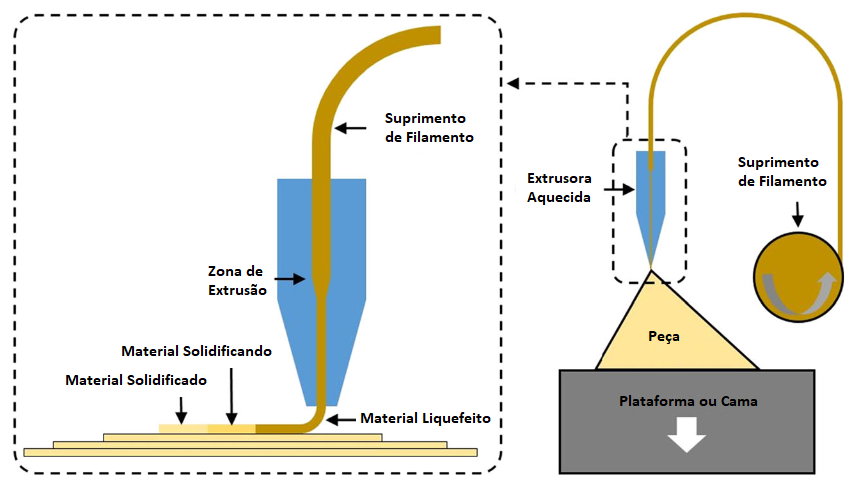
\includegraphics[width=0.7\textwidth]{bikas2015FDM}

    {\footnotesize Fonte:Adaptado de \citeauthor{bikas16}, \citeyear{bikas16}}
    \label{fig:fdm_ex}
    \end{center}
\end{figure}
\end{frame}

\begin{frame}
  \frametitle{\insertsubsection}
  \begin{figure}[H]
    \centering
    \caption{Indicação dos componentes de uma impressora 3D}
    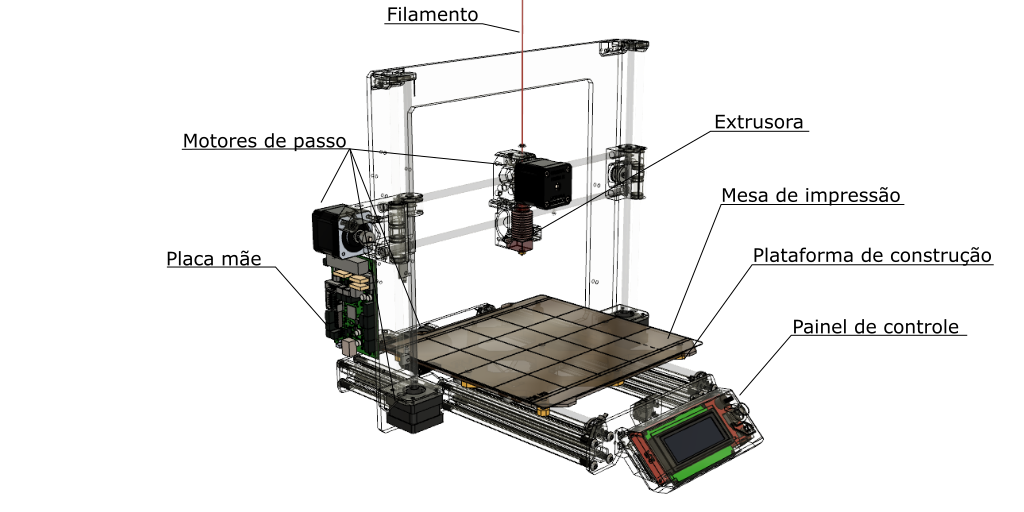
\includegraphics[width=0.8\textwidth]{printer_components}
    \label{fig:impressora3d_comp}
  \end{figure}
\end{frame}

\subsection{\insertsectionnumber .\insertsubsectionnumber . Geração do Modelo 3D digital}
\begin{frame}
  \frametitle{\insertsubsection}
  \begin{itemize}
    \item \textit{Computer Aided Design} (CAD)
    \item Escultura digital
    \item Escaneamento 3D
  \end{itemize}
\end{frame}

\subsection{\insertsectionnumber .\insertsubsectionnumber . Geração de Comando}
\begin{frame}
  \frametitle{\insertsubsection}
  \begin{figure}[H]
    \centering
    \caption{Interface do fatiador PrusaSlicer}
    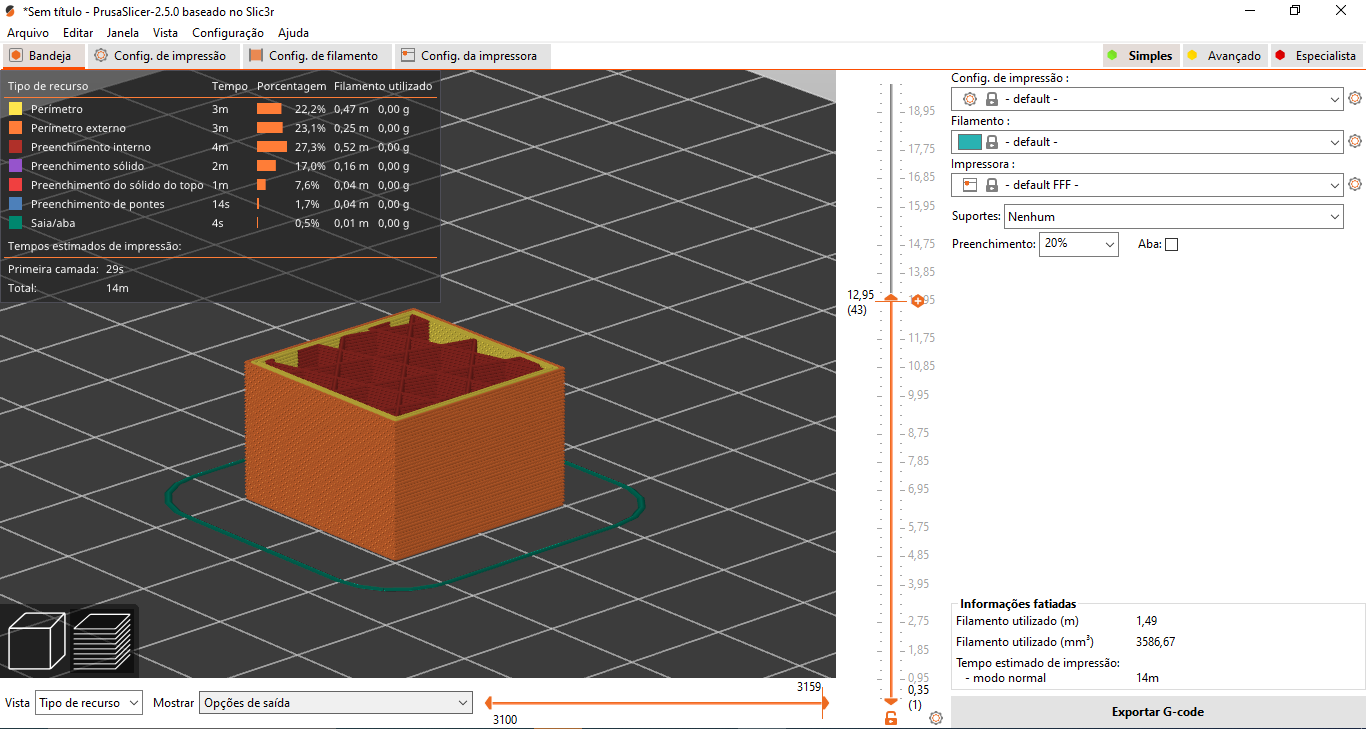
\includegraphics[width=0.8\textwidth]{slicer_inter}
    \label{fig:slicer_inter}
  \end{figure}
\end{frame}

\begin{frame}
  \frametitle{\insertsubsection}
  Exemplos de comandos Gcode
  \begin{itemize}
    \item M104 S200           | Define a temperatura da extrusora
    \item G21                 | Define a unidade como milímetro
    \item G1 X10 Y10 F5000    | Realiza um movimento nos eixos do comando
    \item G1 F1000            | Define a velocidade desejada para os movimentos subsequentes
    \item G1 X10.5 Y9.5 E1.5  | Realiza um movimento nos eixos do comando
    \item G1 X0 Y0 Z0.2 E0    | Realiza um movimento nos eixos do comando 
  \end{itemize}
\end{frame}

\subsection{\insertsectionnumber .\insertsubsectionnumber . Geração de Trajetória}
\begin{frame}
  \frametitle{\insertsubsection}
  \begin{figure}[H]
    \centering
    \caption{Perfil de velocidade - Curva trapezoidal de velocidade}
    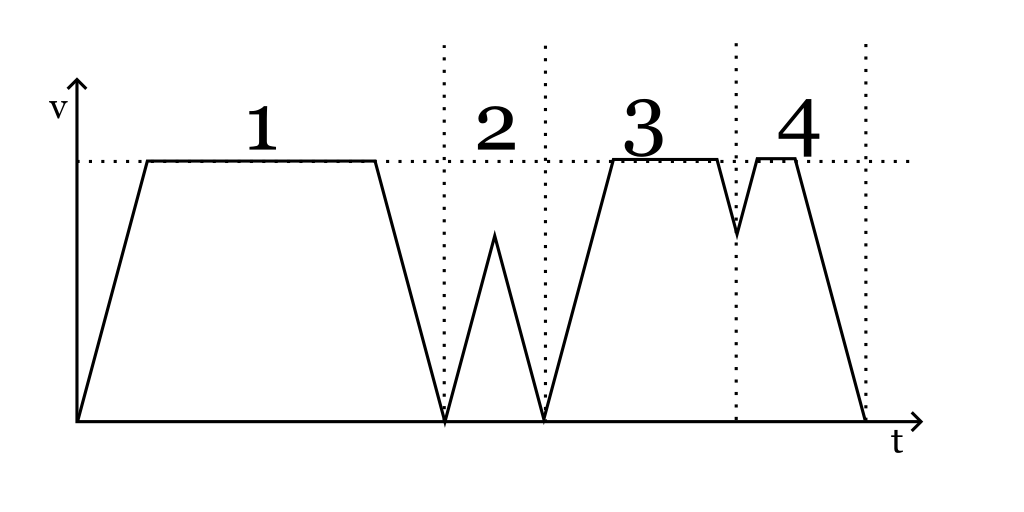
\includegraphics[scale=0.5]{trap_triang}
    \label{fig:trap_triang}
  \end{figure}
\end{frame}

\subsection{\insertsectionnumber .\insertsubsectionnumber . Controle Feedforward}
\begin{frame}
  \frametitle{\insertsubsection}
  O controle \textit{Feedforward} é uma abordagem utilizada em sistemas automáticos, destinada a antecipar e corrigir possíveis perturbações que possam interferir em um sistema a partir de um modelo da planta.
  \begin{itemize}
    \item Possui característica preditiva ao invés de corretiva.
    \item Não necessita de sensores e outros componentes adicionais.
    \item Impressão 3D possui poucas interferências externas à própria impressora.
  \end{itemize}
\end{frame}

\subsection{\insertsectionnumber .\insertsubsectionnumber . \textit{Input Shaping}}
\begin{frame}
  \frametitle{\insertsubsection}
  \begin{figure}[H]
    \centering
    \caption{Comparação da resposta ao degrau e da resposta a escada}
    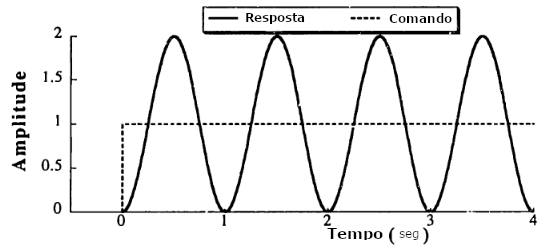
\includegraphics[width=0.45\textwidth]{inputshaperstepresponse1order}
    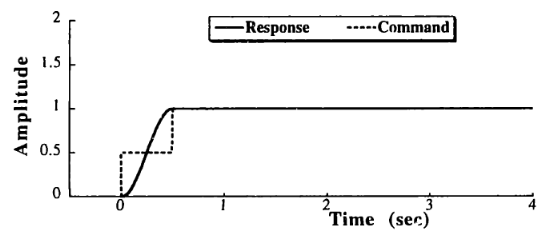
\includegraphics[width=0.45\textwidth]{inputshaperstarcasepresponse}

    {\footnotesize Fonte: Adaptado de \citeauthor{singhose97}, \citeyear{singhose97}}
    \label{fig:degr_vs_esc}
  \end{figure}
\end{frame}

%Conceitos importantes para metodos de controle%

\subsection{\insertsectionnumber .\insertsubsectionnumber . Espaço de Estados}

\begin{frame}
  \frametitle{\insertsubsection}

    \begin{equation}
      \label{eq:edo_ex}
      m \ddot x+c \dot x+kx = f(t)
  \end{equation}

  \begin{equation}
      \label{eq:espaco_de_estados_ex}
      \begin{bmatrix}
          \dot x \\
          \ddot x
      \end{bmatrix}
      =
      \begin{bmatrix}
          0 & 1 \\
          k/m & c/m
      \end{bmatrix}
      \begin{bmatrix}
          x \\
          \dot x
      \end{bmatrix}
      +
      \begin{bmatrix}
          0 \\
          1
      \end{bmatrix}
      f(t)
  \end{equation}
\end{frame}

\subsection{\insertsectionnumber .\insertsubsectionnumber . Programação não linear}

\begin{frame}
  \frametitle{\insertsubsection}

  \begin{columns}
    \begin{column}{.6\textwidth}
      \begin{figure}[H]
        \centering
        \caption{Ilustração Segmentação Cúbica}
        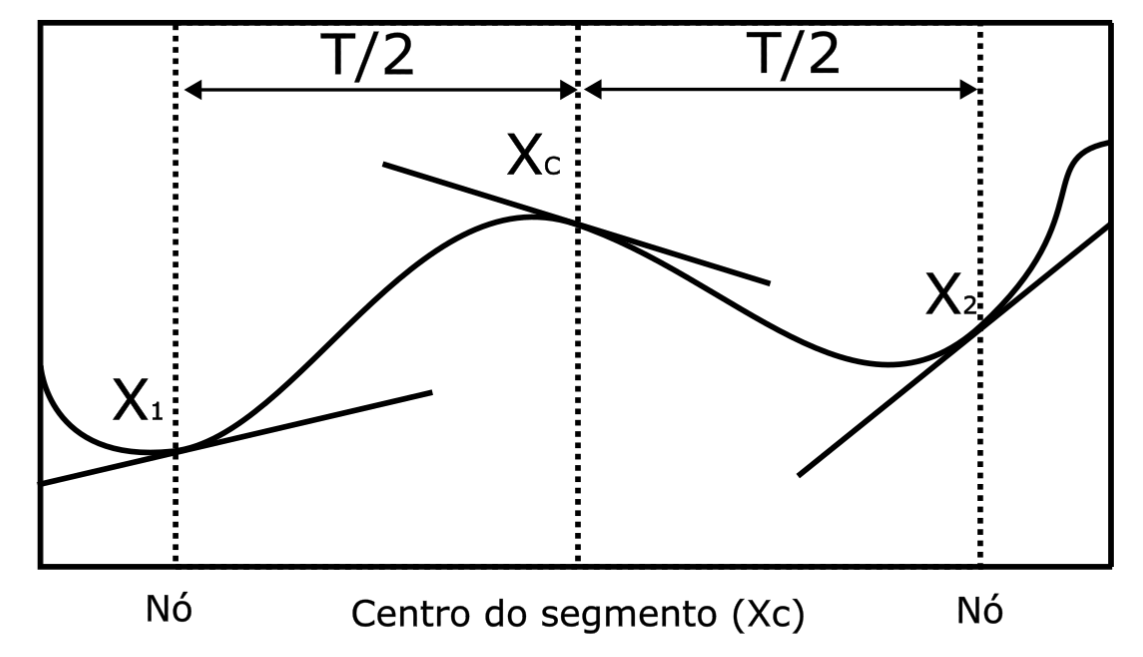
\includegraphics[width=1\textwidth]{hargraves_func}
    
        {\footnotesize Fonte: Adaptado de \citeauthor{hargraves87}, \citeyear{hargraves87}}
        \label{fig:hargraves_fun}
      \end{figure}
    \end{column}
    \begin{column}{.45\textwidth}
      \begin{equation}
        \label{eq:state_center_segment}
        x_c = \frac{x_{1} + x_{2}}{2} + T\frac{f_{1} - f_{2}}{8}
      \end{equation}
    
      \begin{equation}
        \label{eq:state_dot_center_segment}
        \dot{x_{c}} = -3\frac{x_{1} + x_{2}}{2T} + \frac{f_{1} + f_{2}}{4}
      \end{equation}
    
      \begin{equation}
        \label{eq:defect_calc}
        \Delta = f_c - \dot{x_c}
      \end{equation}
    
      \begin{equation}
        \label{eq:input_value_center_segment}
        u_c = \frac{u_1 + u_2}{2}
      \end{equation}
    \end{column}
  \end{columns}
\end{frame}

\section{\insertsectionnumber . Metodologia}
\begin{frame}
  \frametitle{\insertsection}
  \begin{figure}[H]
    \centering
    \caption{Fluxograma geral das etapas para o controle de trajetória}
    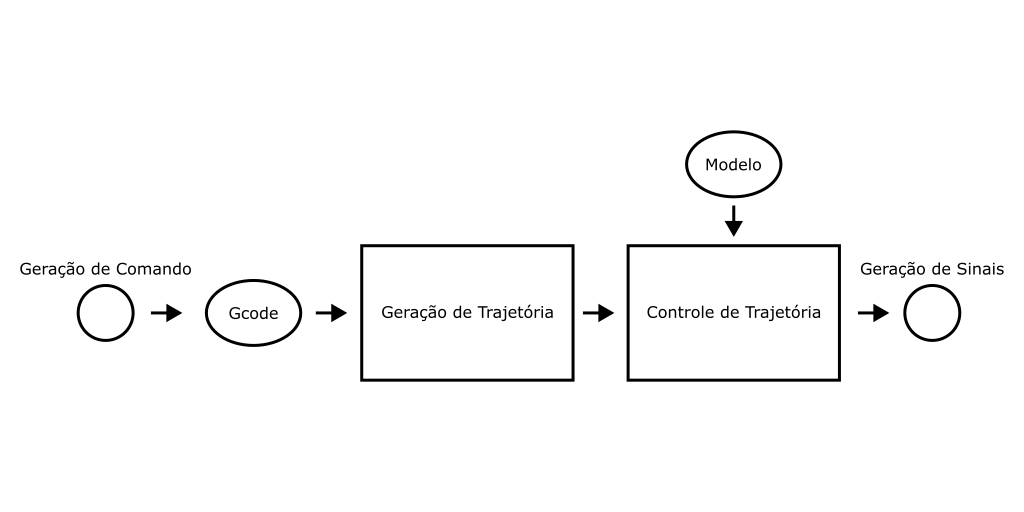
\includegraphics[width=.9\textwidth]{fluxo_geral}
  
    \label{fig:fluxo_geral}
  \end{figure}
\end{frame}

\subsection{\insertsectionnumber .\insertsubsectionnumber . Geração de Trajetória}

\begin{frame}
  \frametitle{\insertsubsection}
  \begin{figure}[H]
    \centering
    \caption{Curva de velocidade trapezoidal}
    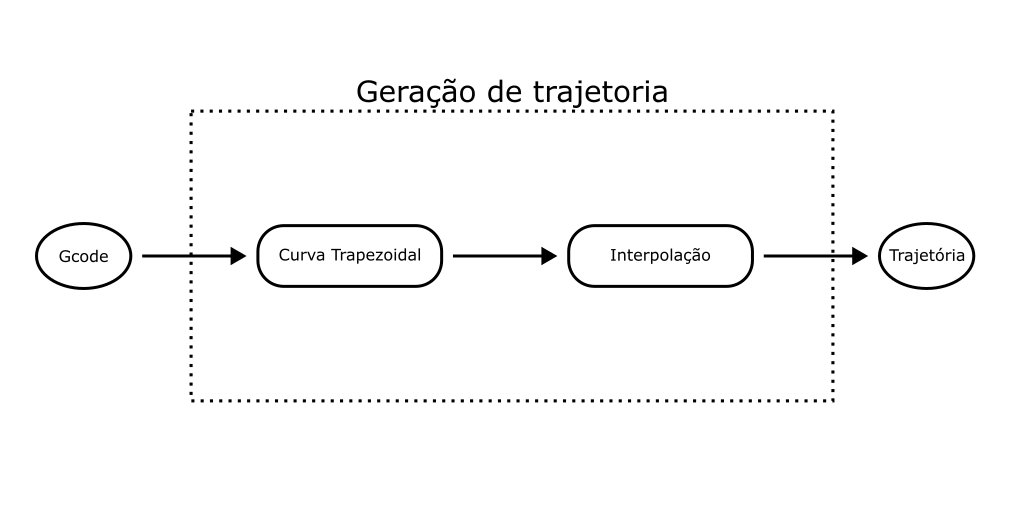
\includegraphics[width=.9\textwidth]{geracao_de_trajetoria}

    \label{fig:geracao_de_trajetoria}
  \end{figure}
\end{frame}

\begin{frame}
  \frametitle{\insertsubsection}
  \begin{columns}
    \begin{column}{.5\textwidth}
      \begin{figure}[H]
        \centering
        \caption{Curva de velocidade triangular}
        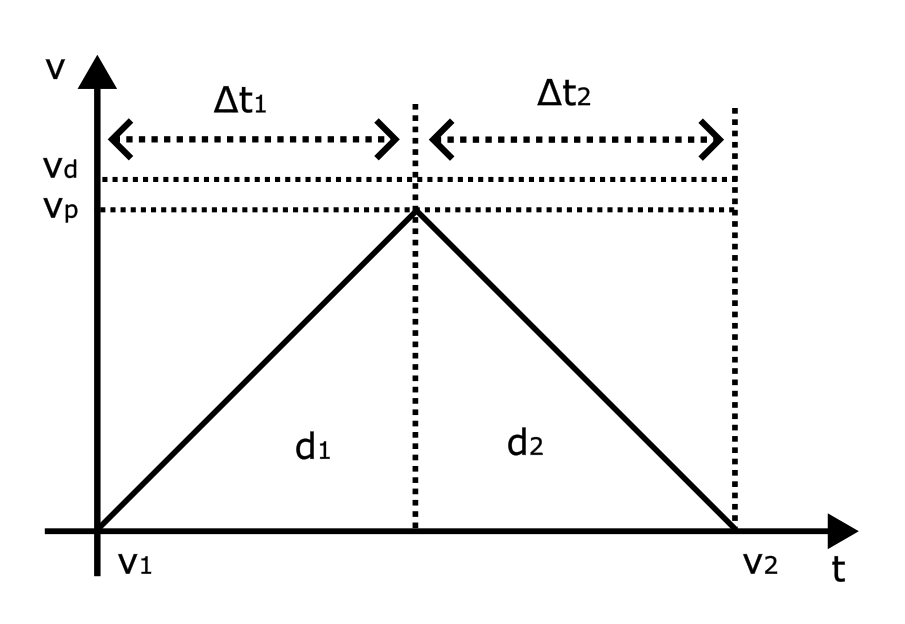
\includegraphics[width=1\textwidth]{triang_curv}

        \label{fig:triang_curv}
      \end{figure}
    \end{column}
    \begin{column}{.45\textwidth}
      \begin{equation}
        \label{eq:v_p}
        v_p = \sqrt{\frac{(v_1^2+v_2^2)}{2}+a d}
      \end{equation}
      \begin{equation}
        \label{eq:des_seg_1_tri}
        d_1 = \frac{(v_p^2-v_1^2)}{(2 a)}
      \end{equation}
      
      \begin{equation}
        \label{eq:des_seg_2_tri}
        d_2 = \frac{(v_2^2-v_p^2)}{(2 a)}
      \end{equation}
      
      \begin{equation}
        \label{eq:dt_seg_1_tri}
        t_1 = \frac{(v_p-v_1)}{a}
      \end{equation}
      
      \begin{equation}
        \label{eq:dt_seg_2_tri}
        t_2 = \frac{(v_2-v_p)}{a}
      \end{equation}
    \end{column}
  \end{columns}
\end{frame}

\begin{frame}
  \frametitle{\insertsubsection}
  \begin{figure}[H]
    \centering
    \caption{Curva de velocidade trapezoidal}
    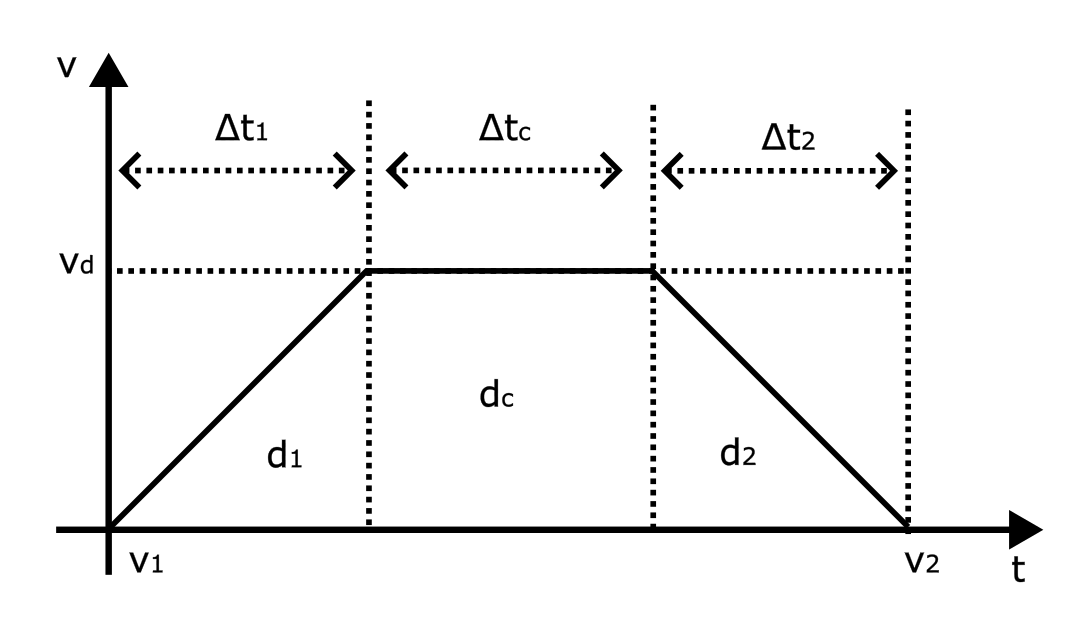
\includegraphics[width=.8\textwidth]{trap_curv}
    \label{fig:trap_curv}
  \end{figure}
\end{frame}

\begin{frame}
  \frametitle{\insertsubsection}
  \begin{columns}
    \begin{column}{.45\textwidth}
      
      \begin{equation}
        \label{eq:des_seg_1_trap}
        d_1 = \frac{(v_d^2-v_1^2)}{(2 a)}
      \end{equation}

      \begin{equation}
        \label{eq:des_seg_2_trap}
        d_2 = \frac{(v_2^2-v_d^2)}{(2 a)}
      \end{equation}

      \begin{equation}
        \label{eq:des_seg_c_trap}
        d_c = d-(d_1+d_2)
      \end{equation}
    \end{column}
    \begin{column}{.45\textwidth}
      
      \begin{equation}
        \label{eq:dt_seg_1_trap}
        \Delta t_1 = \frac{(v_d-v_1)}{a}
      \end{equation}

      \begin{equation}
        \label{eq:dt_seg_2_trap}
        \Delta t_2 = \frac{(v_2-v_d)}{a}
      \end{equation}

      \begin{equation}
        \label{eq:dt_seg_c_trap}
        \Delta t_c = \frac{d_c}{v_d}
      \end{equation}
    \end{column}
  \end{columns}
\end{frame}

\subsection{\insertsectionnumber .\insertsubsectionnumber . Modelagem Dinâmica de uma Impressora 3D}

\begin{frame}
  \frametitle{\insertsubsection}
  \begin{itemize}
    \item Correias definidas como uma combinação de mola e amortecedor.
    \item Simplificação da extrusora como corpo rígido e uniforme.
    \item Limites de movimento de 0 a 200 mm para os eixos X e Y.
    \item Impressora cartesiana, eixos ortogonais e independentes.
    \item O estado inicial dos pontos relevantes parte do repouso.
\end{itemize}
\end{frame}

\begin{frame}
  \frametitle{\insertsubsection}
  \begin{figure}[H]
    \centering
    \caption{Modelo simplificado impressora 3D}
    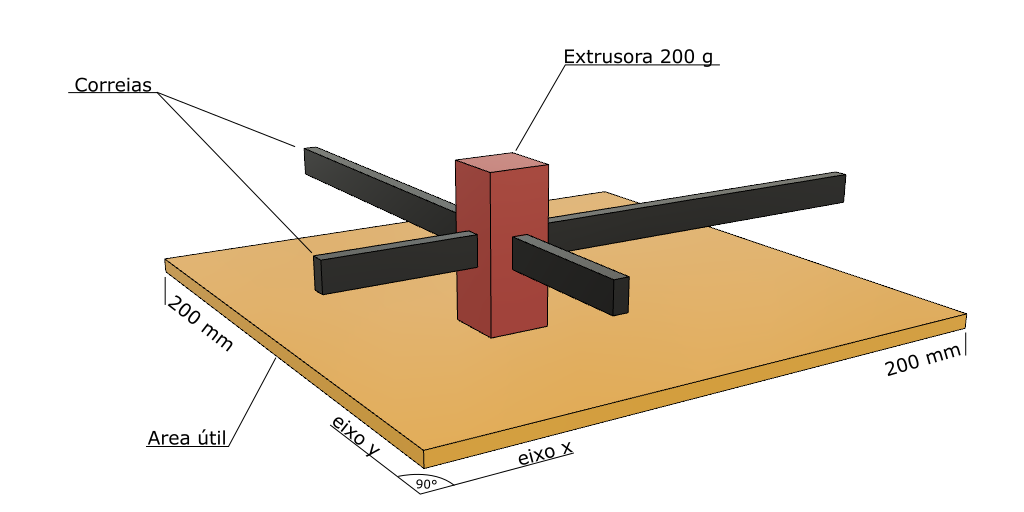
\includegraphics[width=0.6\textwidth]{simple_model}
    \label{fig:simple_model}
  \end{figure}
\end{frame}

\begin{frame}
  \frametitle{\insertsubsection}
  \begin{equation}
    \label{eq:mov_impressora_2}
    \ddot{x_p} = \frac{c}{m}(\dot{x_b} - \dot{x_p}) + \frac{k}{m}(x_b - x_p) 
  \end{equation}
  \begin{figure}[H]
    \centering
    \caption{Modelagem de 1 eixo}
    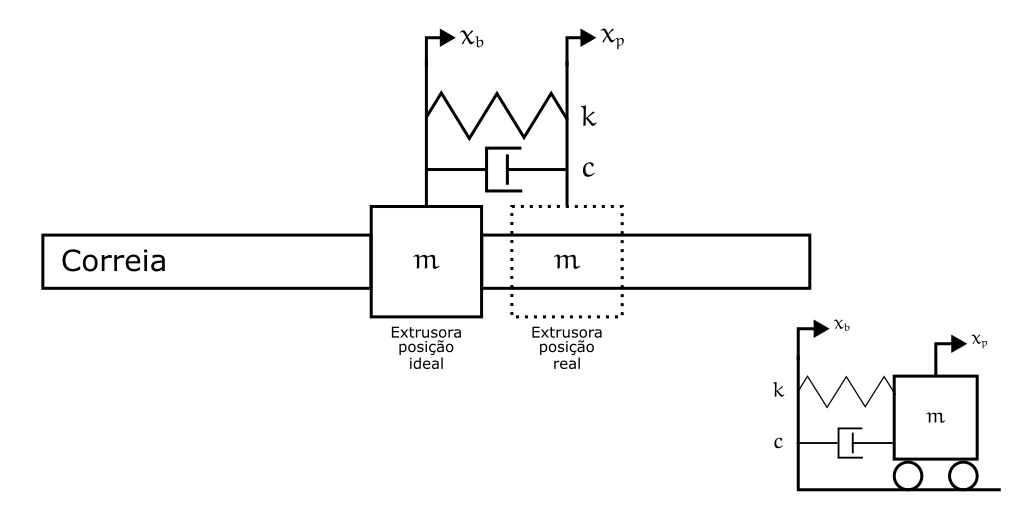
\includegraphics[width=.7\textwidth]{model_1_axis}

    \label{fig:model_1_axis}
  \end{figure}
\end{frame}

\begin{frame}
  \frametitle{\insertsubsection}
  \begin{figure}[H]
    \centering
    \caption{Modelagem dos eixos x e y}
    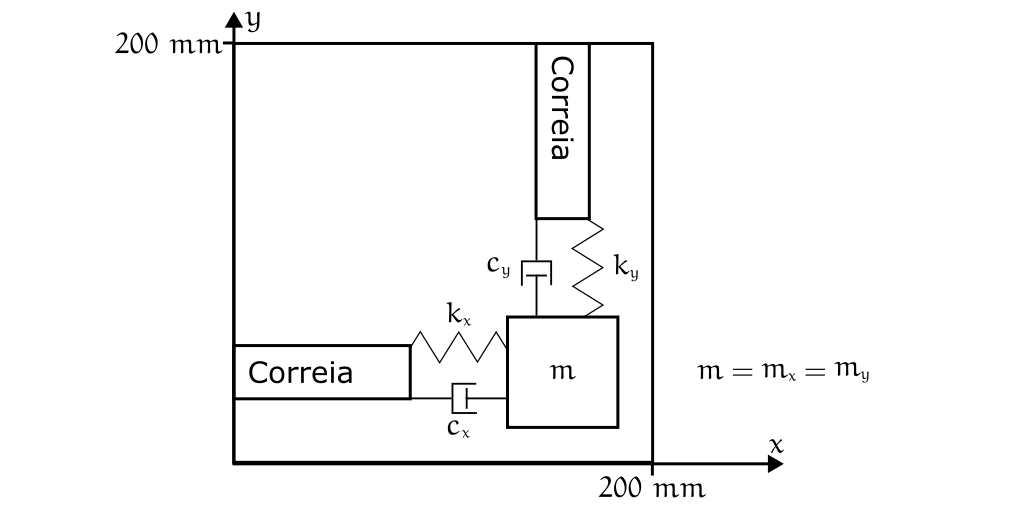
\includegraphics[scale=0.4]{model_2_axis}

    \label{fig:model_2_axis}
  \end{figure}
\end{frame}

\begin{frame}
  \frametitle{\insertsubsection}
  
  \begin{equation}
    \label{eq:freq_nat}
    \omega = \sqrt{\frac{k}{m}}
  \end{equation}
  
  \begin{equation}
    \label{eq:amort}
    \zeta = \frac{c}{2mk}
  \end{equation}
  
  \begin{equation}
    \label{eq:equation_simpl}
    \ddot{x_p} = 2 \zeta \omega(\dot{x_b} - \dot{x_p}) + \omega ^2(x_b - x_p)
  \end{equation}
\end{frame}

\subsection{\insertsectionnumber .\insertsubsectionnumber . Representação em Espaço de Estados}
\begin{frame}
  \frametitle{\insertsubsection}
  \begin{equation}
    \label{eq:simp_state_space_din_model}
    \dot x = A*x+B*u
  \end{equation}
  
  \begin{equation}
    \label{eq:espaco_de_estados_din_model}
    \begin{bmatrix}
        \dot{x_p} \\
        \dot{y_p} \\
        \ddot{x_p} \\
        \ddot{y_p}
    \end{bmatrix}
    =
    \begin{bmatrix}
        0 & 0 & 1 & 0 \\
        0 & 0 & 0 & 1 \\
        -\omega _x ^2 & 0 & -2 \zeta _x \omega _x & 0 \\
        0 & -\omega _y ^2 & 0 & -2 \zeta _y \omega _y
    \end{bmatrix}
    \begin{bmatrix}
        x_p \\    
        y_p \\
        \dot{x_p} \\    
        \dot{y_p} \\
    \end{bmatrix}
    +
    \begin{bmatrix}
        0 & 0 & 0 & 0 \\
        0 & 0 & 0 & 0 \\
        \omega _x ^2 & 0 & 2 \zeta _x \omega _x & 0 \\
        0 & \omega _y ^2 & 0 & 2 \zeta _y \omega _y
    \end{bmatrix}
    \begin{bmatrix}
        x_b \\
        y_b \\
        \dot{x_b}  \\
        \dot{y_b} 
    \end{bmatrix}
  \end{equation}
\end{frame}

\subsection{\insertsectionnumber .\insertsubsectionnumber . Controle de Trajetória}
\begin{frame}
  \frametitle{\insertsubsection}
  \begin{figure}[H]
    \centering
    \caption{Fluxograma Controle de Trajetória}
    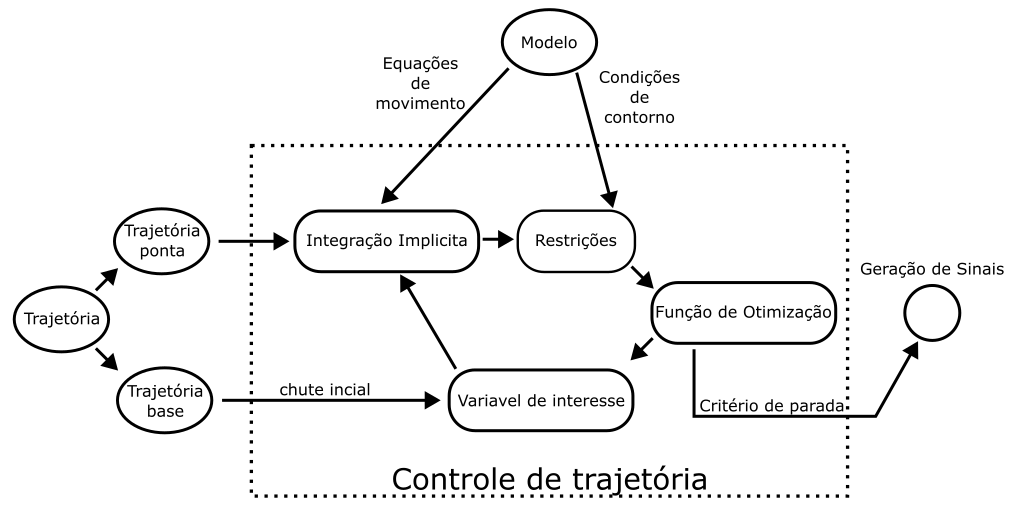
\includegraphics[scale=0.5]{controle_de_trajetoria}

    \label{fig:controle_de_trajetoria}
  \end{figure}
\end{frame}

\subsection{\insertsectionnumber .\insertsubsectionnumber . Restrições}
\begin{frame}
  \frametitle{\insertsubsection}
  \begin{itemize}
    \item Aplica o modelo dinâmico através da programação não linear, minimizando o desvio calculado pela mesma.
    \item Define o estado inicial e final.
    \item Aplica os limites de movimento.
    \item Define o caminho desejado.
  \end{itemize}
\end{frame}

\subsection{\insertsectionnumber .\insertsubsectionnumber . Função de otimização}
\begin{frame}
  \frametitle{\insertsubsection}
  \begin{itemize}
    \item Utiliza o algoritmo de interior-point (encontrando o gradiente da função no ponto) para minimizar o descumprimento das restrições através da modificação da variável de interesse.
    \item Avança iterativamente na direção do gradiente.
    \item Define os critérios de parada.
  \end{itemize}
\end{frame}

\section{\insertsectionnumber . Resultados}

\begin{frame}
  \frametitle{\insertsection}
  Utilização do método de Runge-Kutta para comparação dos efeitos das trajetória da base (com controle e sem controle) na trajetória da ponta (bico da impressora).
  \begin{columns}
    \begin{column}{.4\textwidth}
      \begin{itemize}
        \item Sequência de movimentos para as simulações.
      \end{itemize}
    \end{column}
    \begin{column}{.5\textwidth}
      \begin{figure}[H]
        \centering
        \caption{Movimento base}
        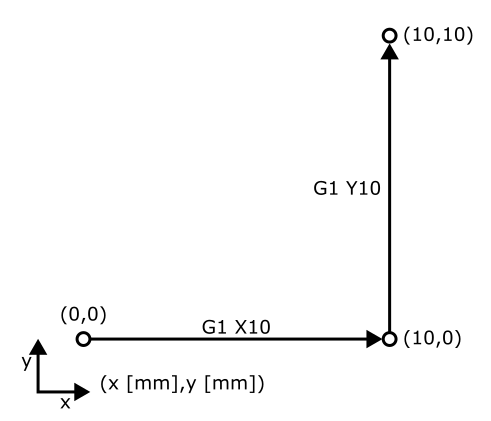
\includegraphics[width=.85\textwidth]{base_mov}
    
        \label{fig:base_mov}
      \end{figure}
    \end{column}
  \end{columns}
\end{frame}

\begin{frame}
  \frametitle{\insertsection}
  \begin{figure}[H]
    \centering
    \caption{Fluxograma geral com os parâmetros.}
    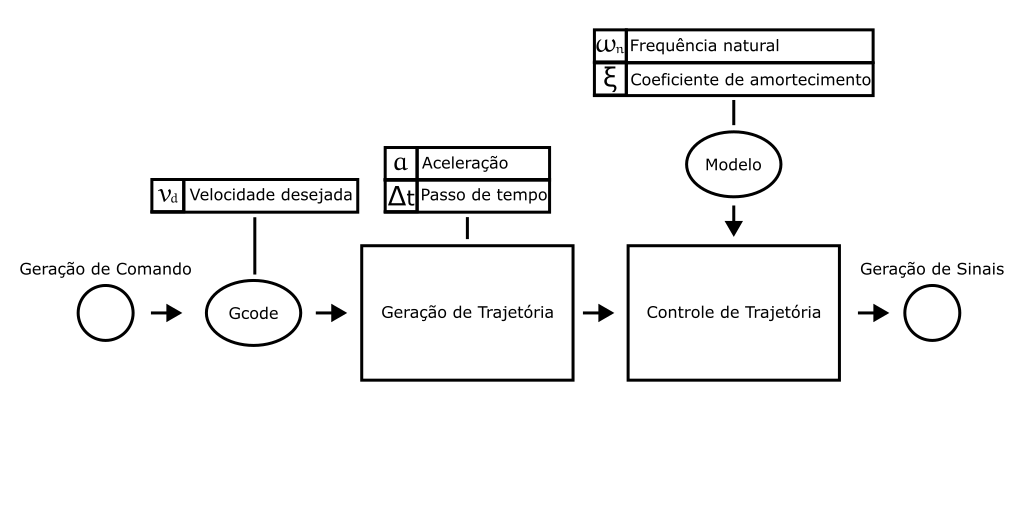
\includegraphics[width=.9\textwidth]{fluxo_geral_var}

    \label{fig:fluxo_geral_var}
\end{figure}
\end{frame}

\subsection{\insertsectionnumber .\insertsubsectionnumber . Simulação Referência}
\begin{frame}
  \frametitle{\insertsubsection}
  \begin{table}
    \begin{center}
    \caption{Valores dos parâmetros utilizados na simulação referência.}
    \label{tab:base_params}
    \begin{tabular}{c c c}
        Parâmetro & Valor & Unidade\\ \hline
        Frequência & 100 & $rad/s$\\
        Coeficiente de amortecimento & 0,5 & - \\
        Aceleração base & 5000 & $mm/s^2$ \\
        Velocidade desejada & 100 & $mm/s$ \\
        Passo de tempo & 0,005 & $s$ \\ \hline
    \end{tabular}
    \end{center}
  \end{table}
\end{frame}

\subsection{\insertsectionnumber .\insertsubsectionnumber . Resultados da Simulação Referência}

\begin{frame}
  \frametitle{\insertsubsection}
  \begin{figure}[H]
    \centering
    \caption{Caminhos da ponta e da base.}
    \subfigure[Sem controle.]{
        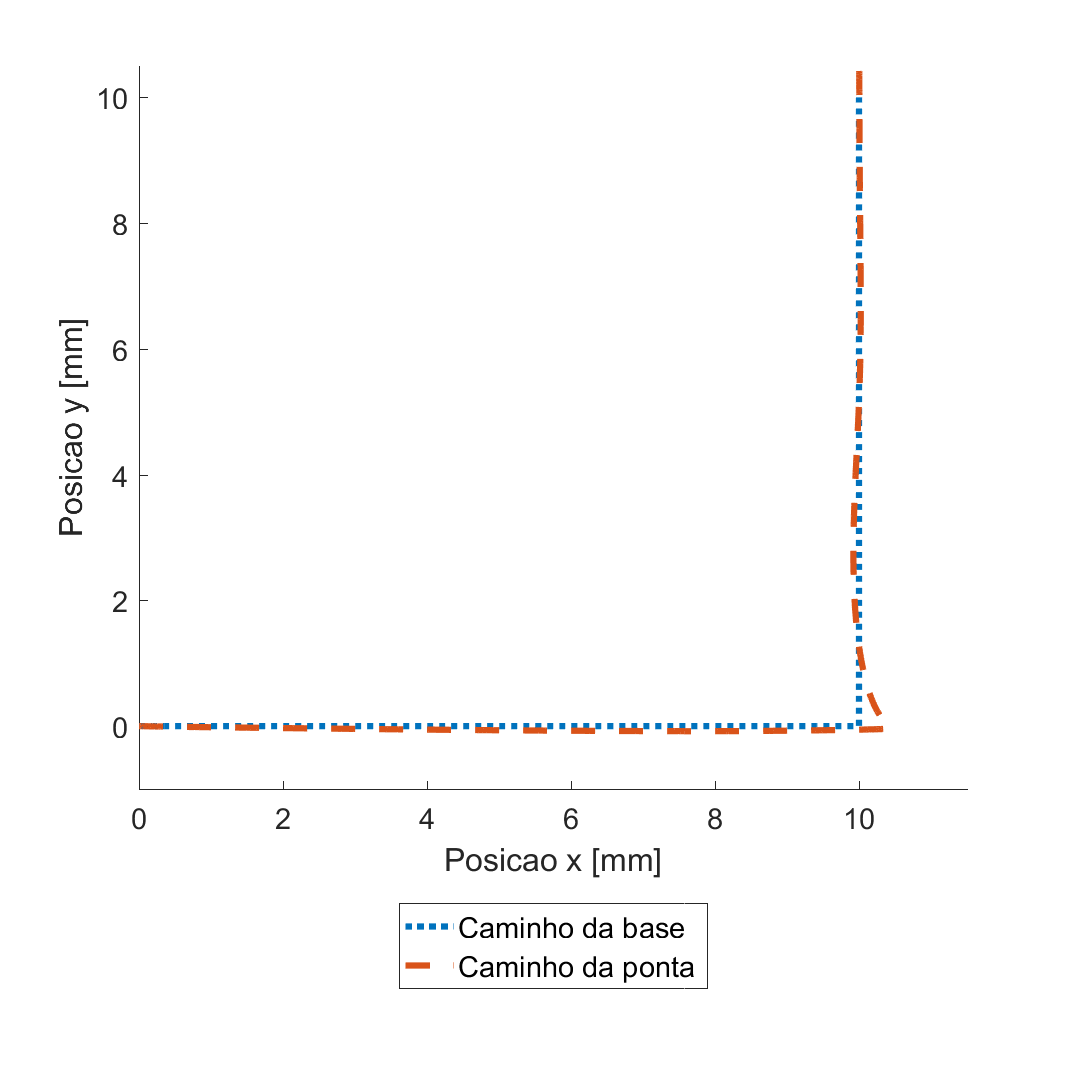
\includegraphics[width=0.38\textwidth]{Sim ref_cam_s.png}
        \label{fig:ref_cam_s}
    }
    \hfill
    \subfigure[Com controle.]{
        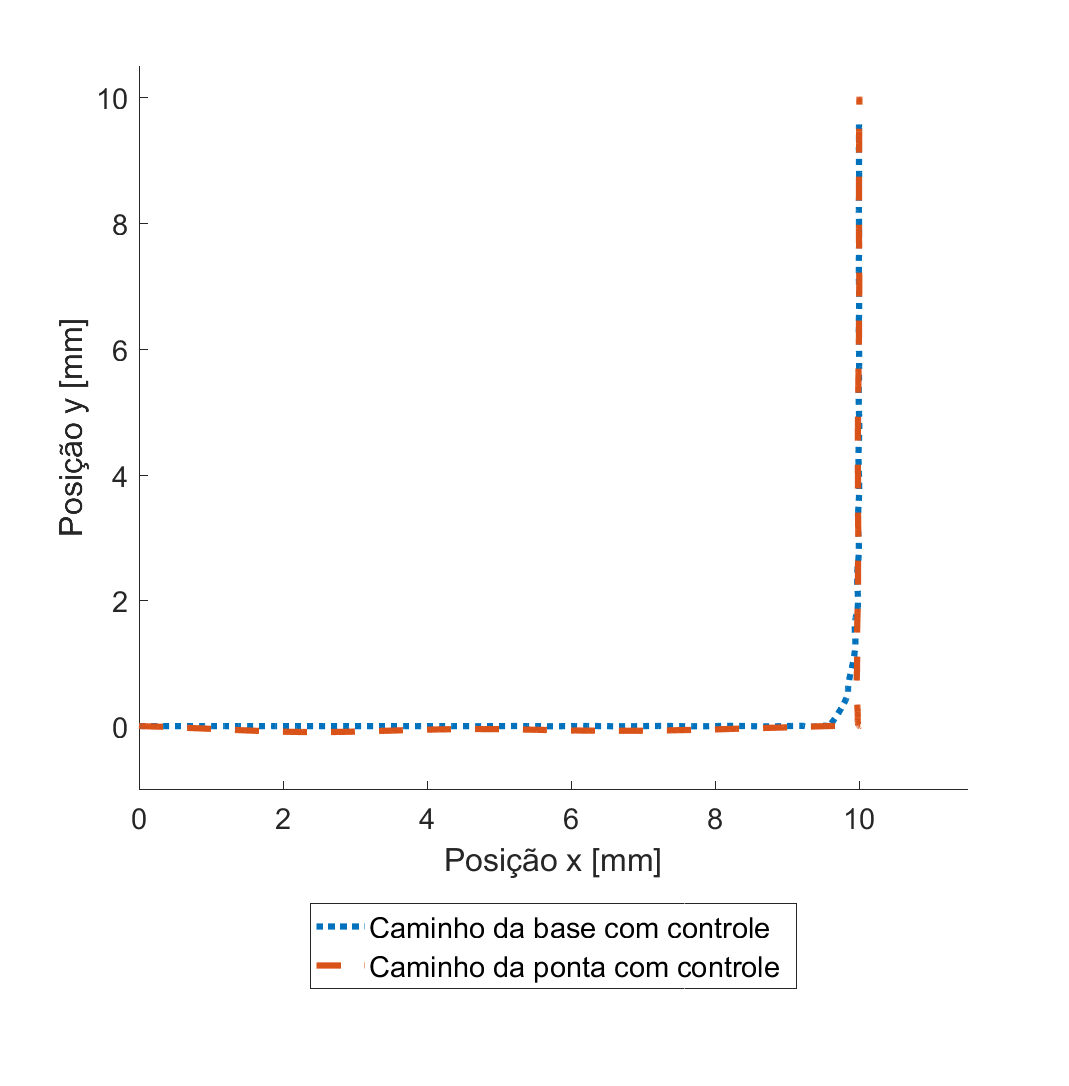
\includegraphics[width=0.38\textwidth]{Sim ref_cam_c.png}
        \label{fig:ref_cam_c}
    }
  \end{figure}
\end{frame}

\begin{frame}
  \frametitle{\insertsubsection}
  \begin{figure}[H]
    \centering
    \caption{Caminhos da ponta e da base - Detalhamento}
    \subfigure[Sem controle.]{
        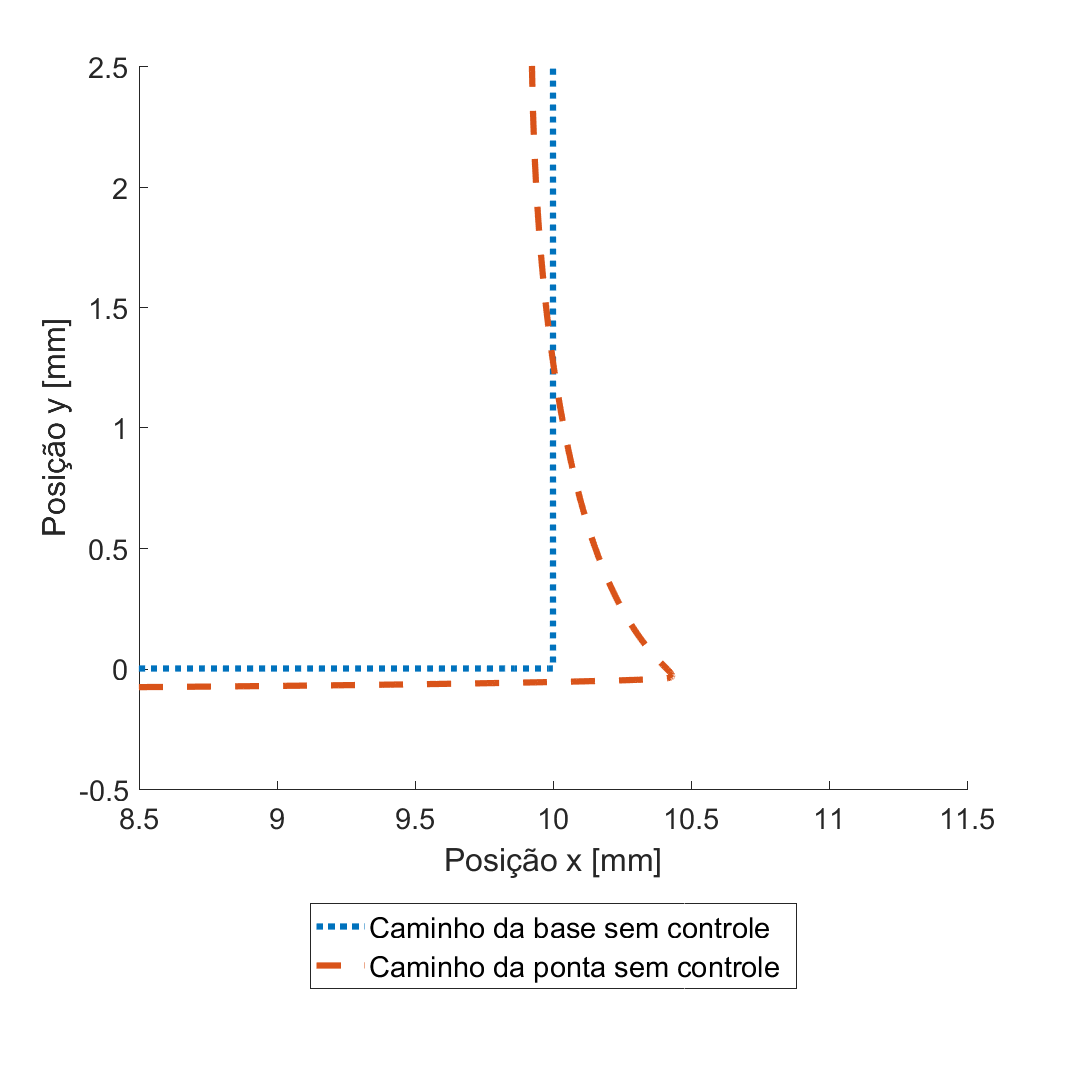
\includegraphics[width=0.38\textwidth]{Sim ref_cam_s_zoom.png}
        \label{fig:ref_cam_s_zoom}
    }
    \hfill
    \subfigure[Com controle.]{
        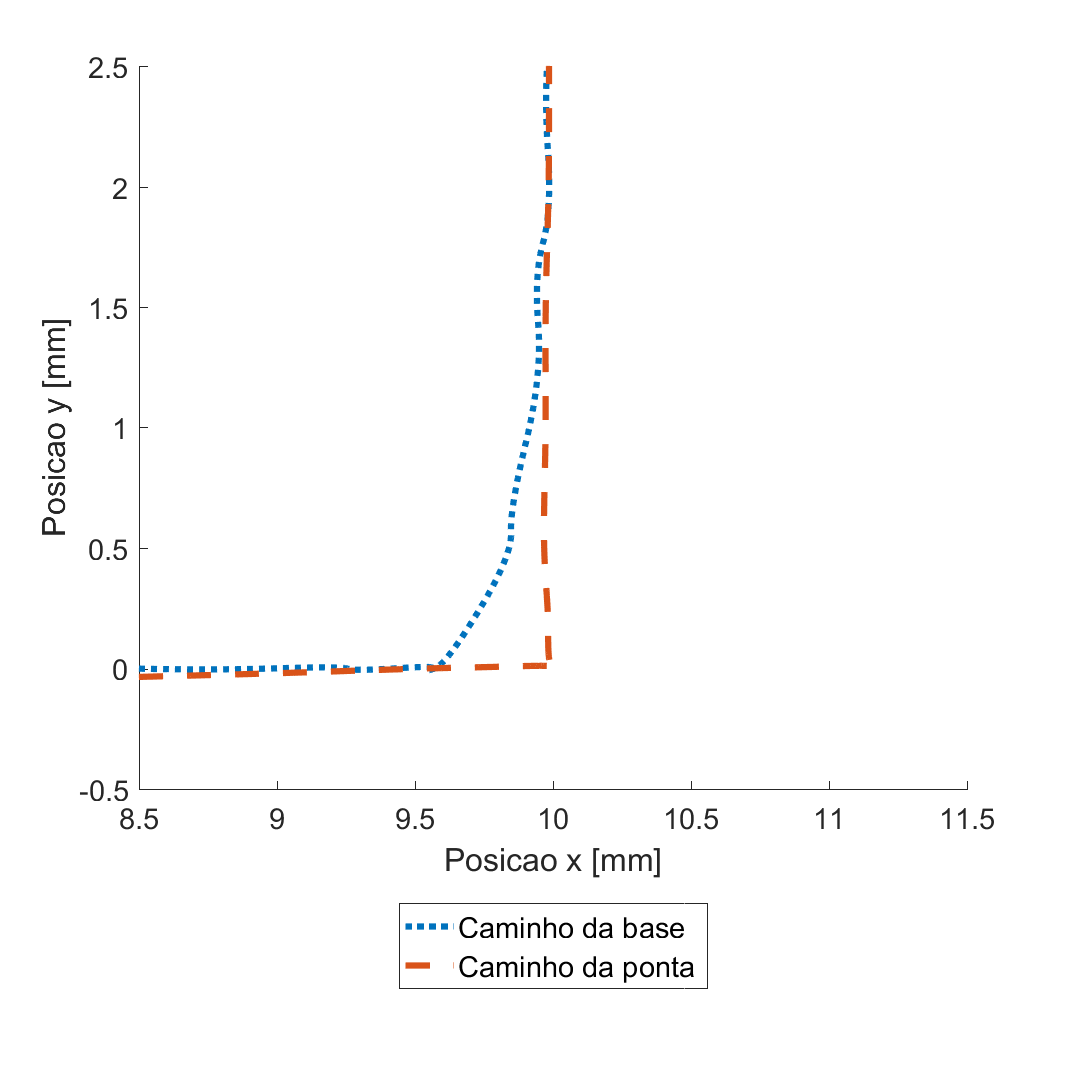
\includegraphics[width=0.38\textwidth]{Sim ref_cam_c_zoom.png}
        \label{fig:ref_cam_c_zoom}
    }
  \end{figure}
\end{frame}

\begin{frame}
  \frametitle{\insertsubsection}
  \begin{figure}[H]
    \centering
    \caption{Deslocamentos da ponta e da base.}
    \subfigure[Sem controle.]{
        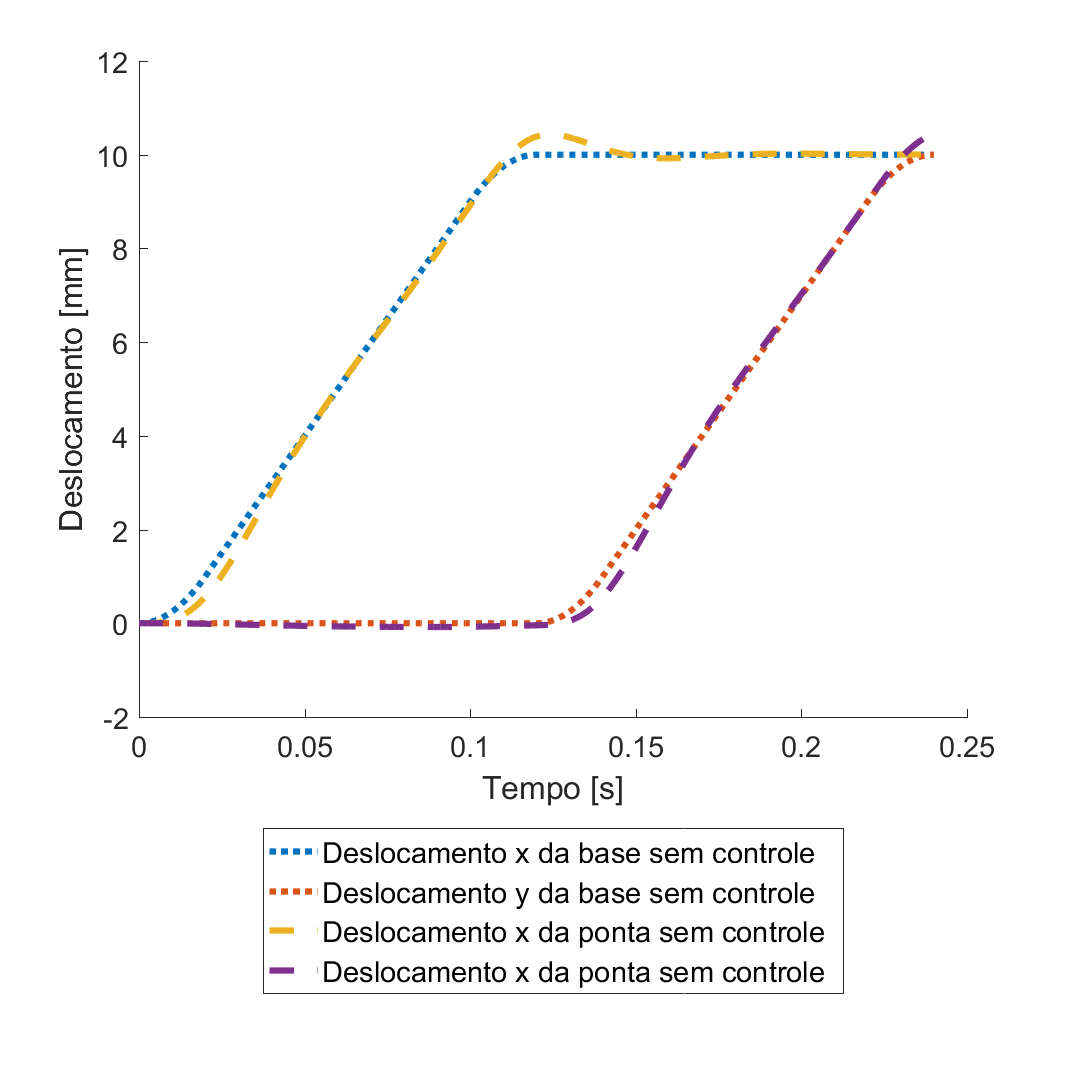
\includegraphics[width=0.38\textwidth]{Sim ref_des_s.png}
        \label{fig:ref_des_s}
    }
    \hfill
    \subfigure[Com controle.]{
        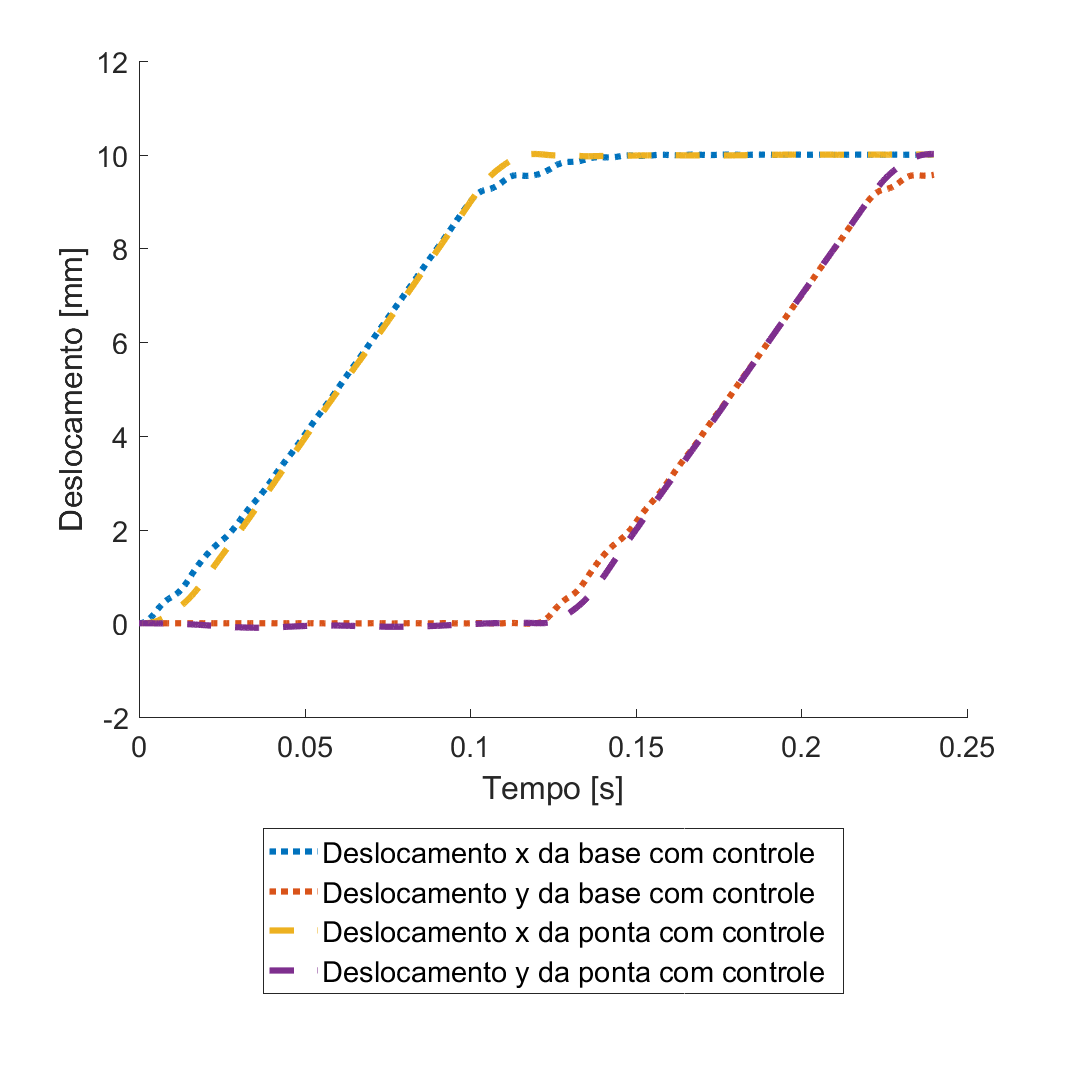
\includegraphics[width=0.38\textwidth]{Sim ref_des_c.png}
        \label{fig:ref_des_c}
    }
    \label{fig:ref_des}
  \end{figure}
\end{frame}

\begin{frame}
  \frametitle{\insertsubsection}
  \begin{figure}[H]
    \centering
    \caption{Velocidades da ponta e da base.}
    \subfigure[Sem controle.]{
        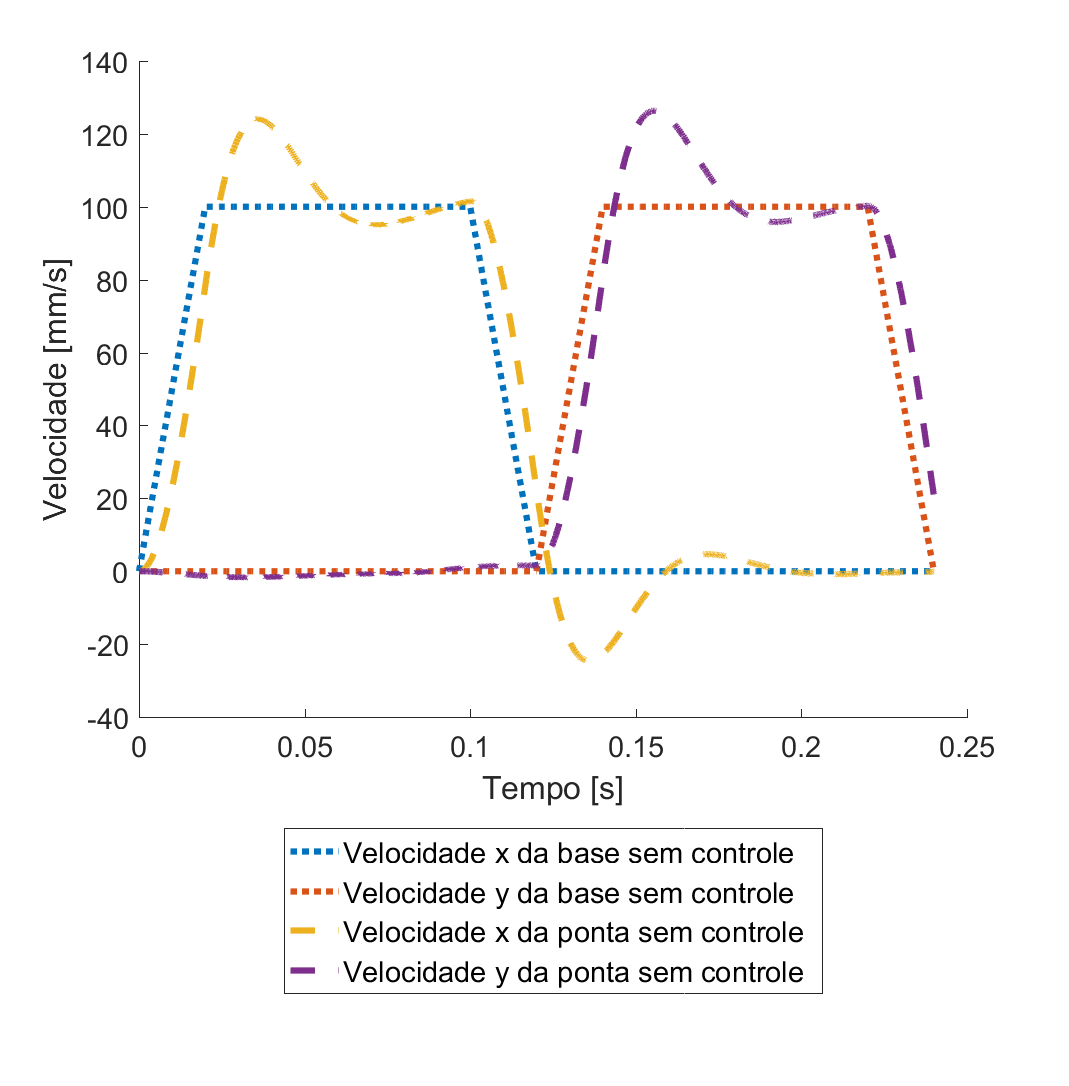
\includegraphics[width=0.38\textwidth]{Sim ref_vel_s.png}
        \label{fig:ref_vel_s}
    }
    \hfill
    \subfigure[Com controle.]{
        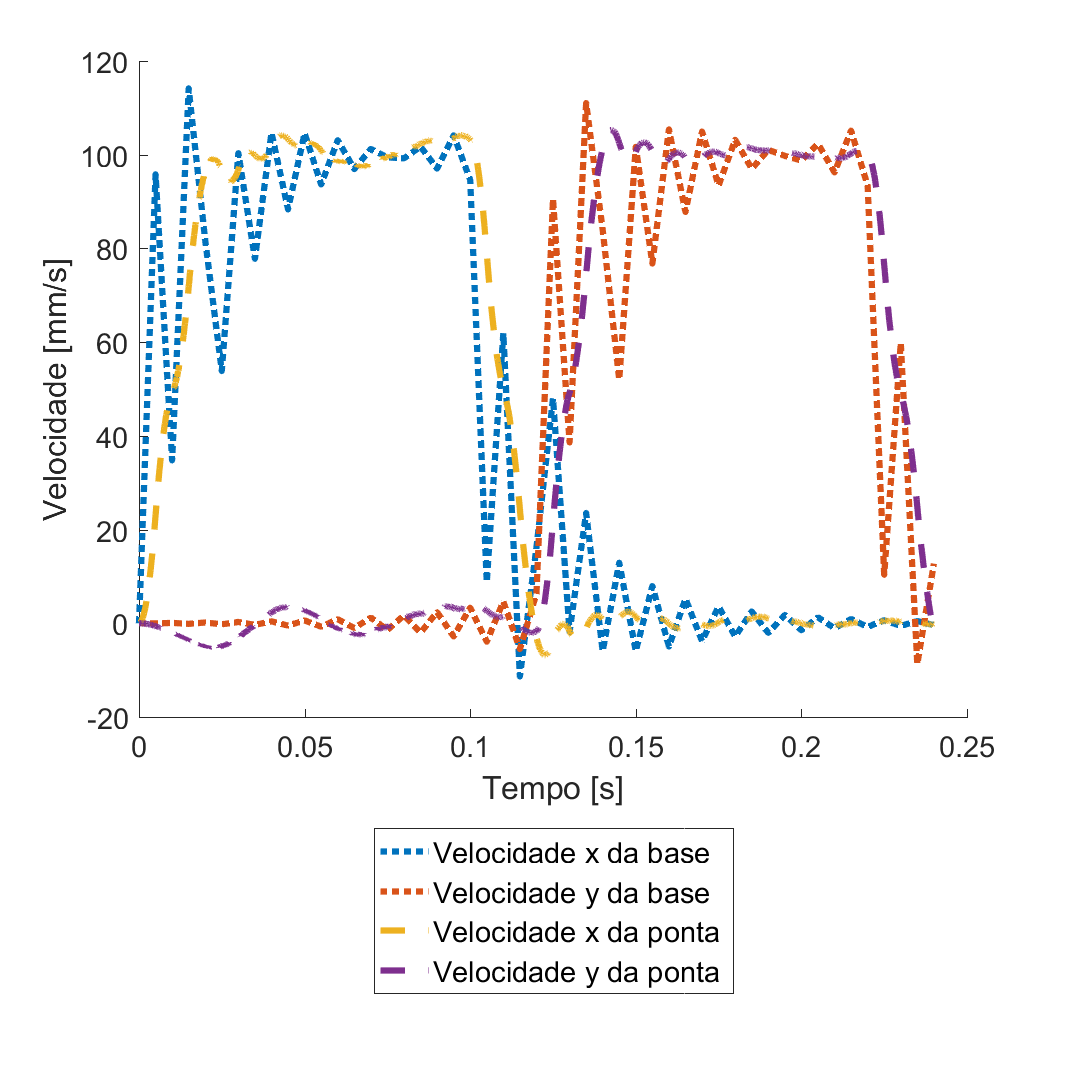
\includegraphics[width=0.38\textwidth]{Sim ref_vel_c.png}
        \label{fig:ref_vel_c}
    }
    \label{fig:ref_vel}
  \end{figure}
\end{frame}

\subsection{\insertsectionnumber .\insertsubsectionnumber . Simulação com Parâmetros Variados}
\begin{frame}
  \frametitle{\insertsubsection}
  \begin{table}
    \begin{center}
    \caption{Parâmetros utilizados nas simulações.}
    \label{tab:sim_params}
    \begin{tabular}{c c c c c}
        Caso & Parâmetro & Valor A & Valor B & Unidade\\ \hline
        1 & Frequência & 50 & 200 & $rad/s$\\
        2 & Coeficiente de amortecimento & 0 & 1 & - \\
        3 & Aceleração base & 1000 & 10000 & $mm/s^2$ \\
        4 & Velocidade desejada & 50 & 200 & $mm/s$ \\
        5 & Passo de tempo & 0,1 & 0,001 & $s$ \\ \hline
    \end{tabular}
    \end{center}
  \end{table}
\end{frame}

\subsection{\insertsectionnumber .\insertsubsectionnumber . Simulação - Variação da Frequência Natural (50$rad/s$ - 200$rad/s$)}

\begin{frame}
  \frametitle{\insertsubsection}
  \begin{figure}[H]
    \centering
    \caption{Caminhos da ponta e da base - Detalhamento (A).}
    \subfigure[Sem controle.]{
        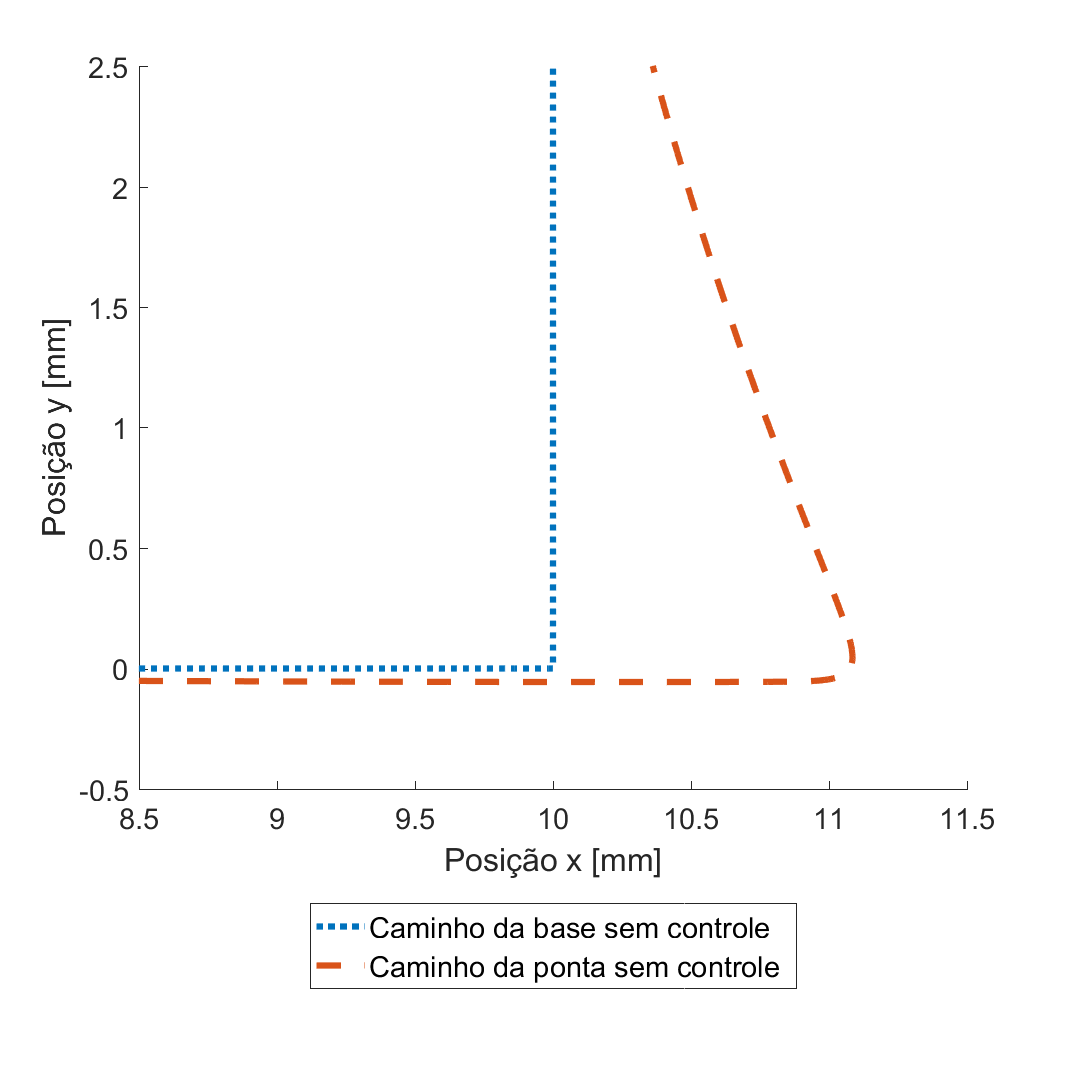
\includegraphics[width=0.38\textwidth]{Sim 1A_cam_s_zoom.png}
        \label{fig:1A_cam_s_zoom}
    }
    \hfill
    \subfigure[Com controle.]{
        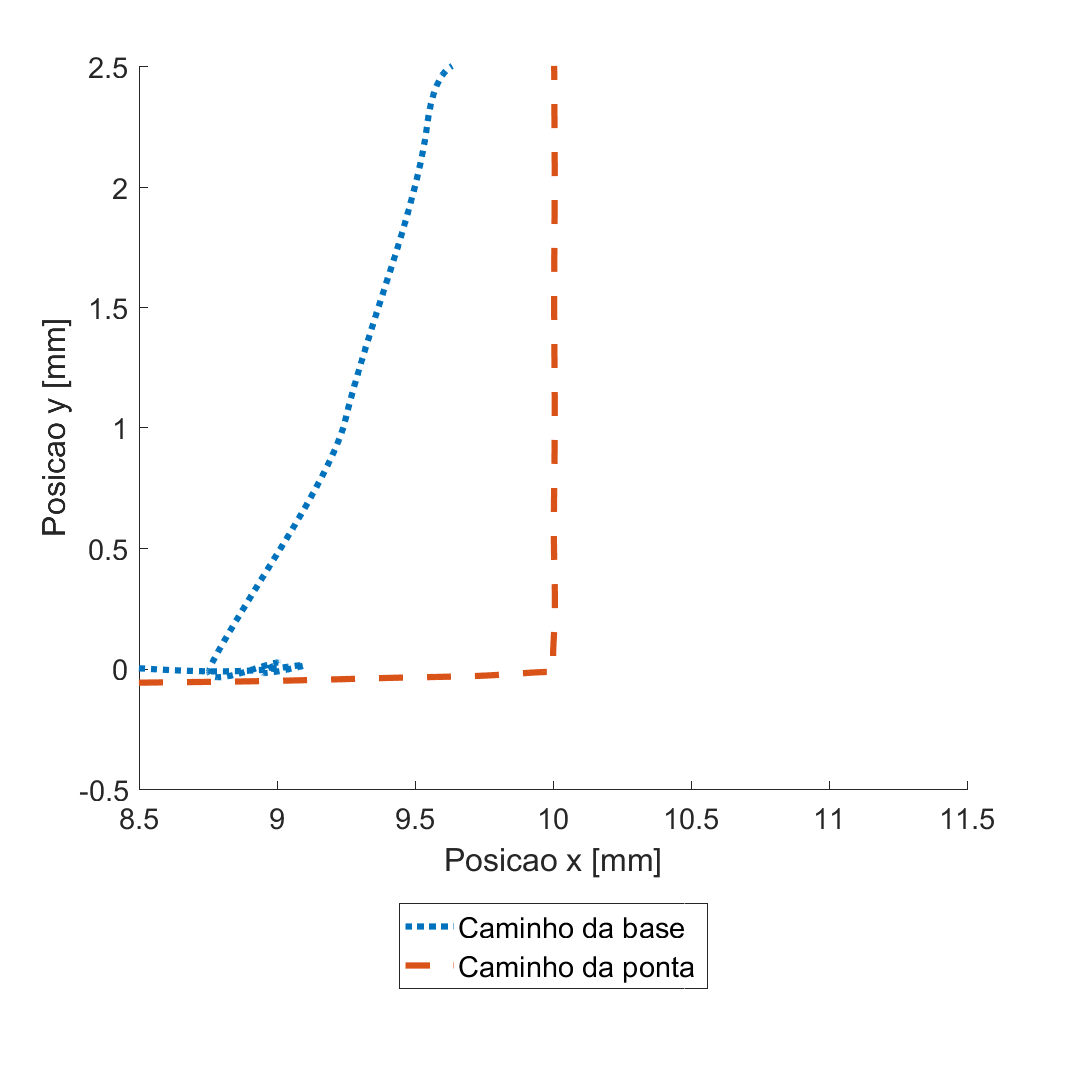
\includegraphics[width=0.38\textwidth]{Sim 1A_cam_c_zoom.png}
        \label{fig:1A_cam_c_zoom}
    }
  \end{figure}
\end{frame}

\begin{frame}
  \frametitle{\insertsubsection}
  \begin{figure}[H]
    \centering
    \caption{Caminhos da ponta e da base - Detalhamento (B)}
    \subfigure[Sem controle.]{
        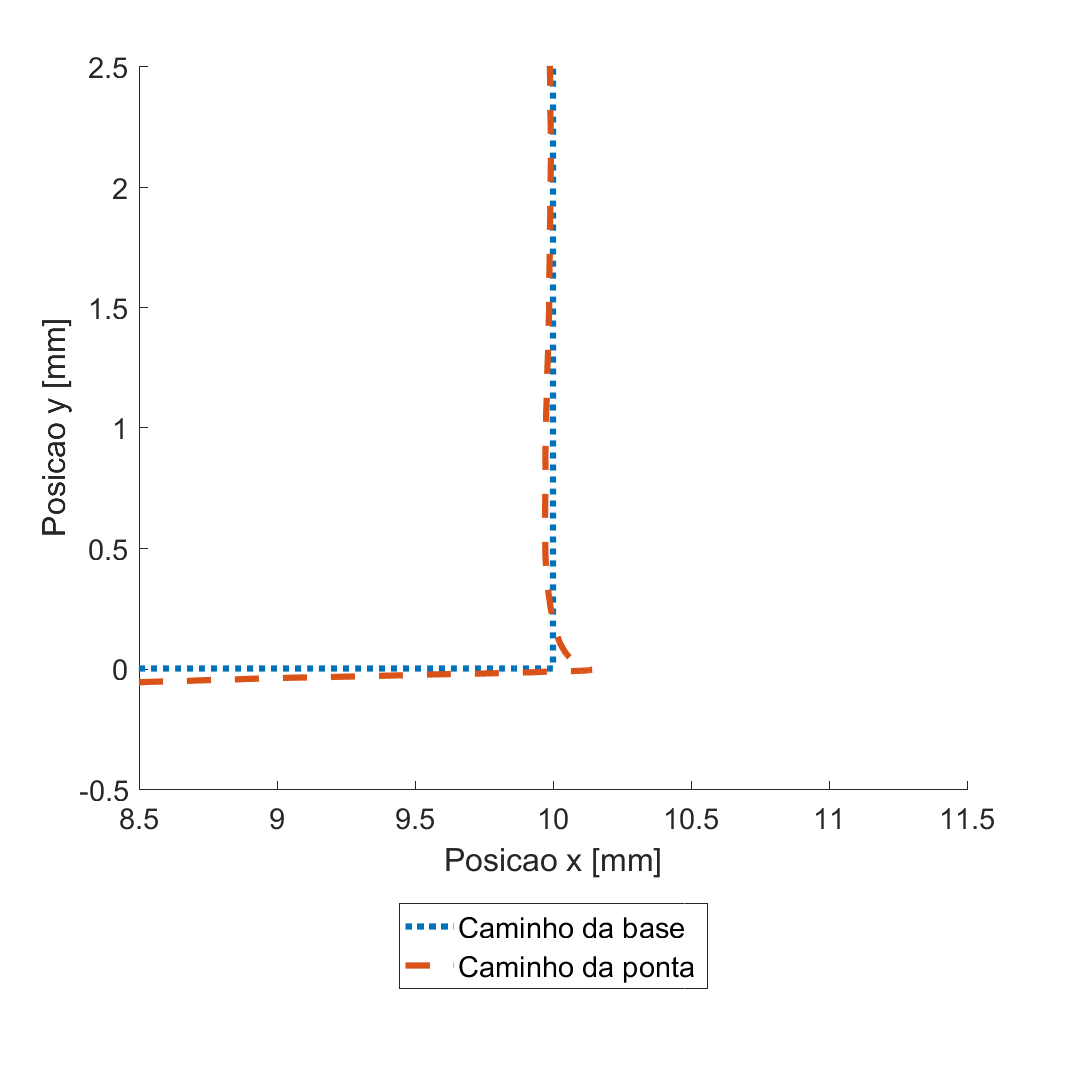
\includegraphics[width=0.38\textwidth]{Sim 1B_cam_s_zoom.png}
        \label{fig:1B_cam_s_zoom}
    }
    \hfill
    \subfigure[Com controle.]{
        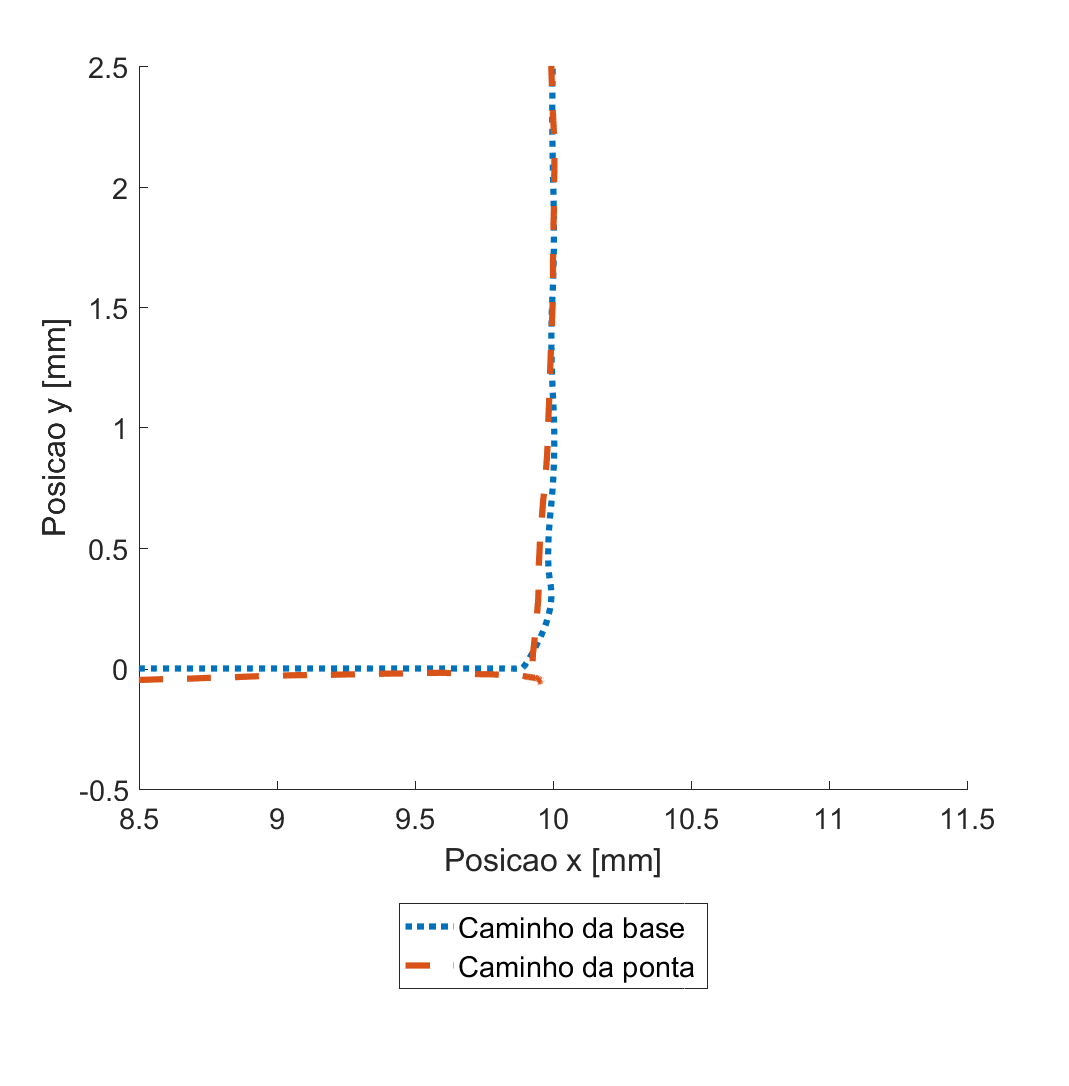
\includegraphics[width=0.38\textwidth]{Sim 1B_cam_c_zoom.png}
        \label{fig:1B_cam_c_zoom}
    }
  \end{figure}
\end{frame}

\begin{frame}
  \frametitle{\insertsubsection}
  \begin{figure}[H]
    \centering
    \caption{Velocidades da ponta e da base (A).}
    \subfigure[Sem controle.]{
        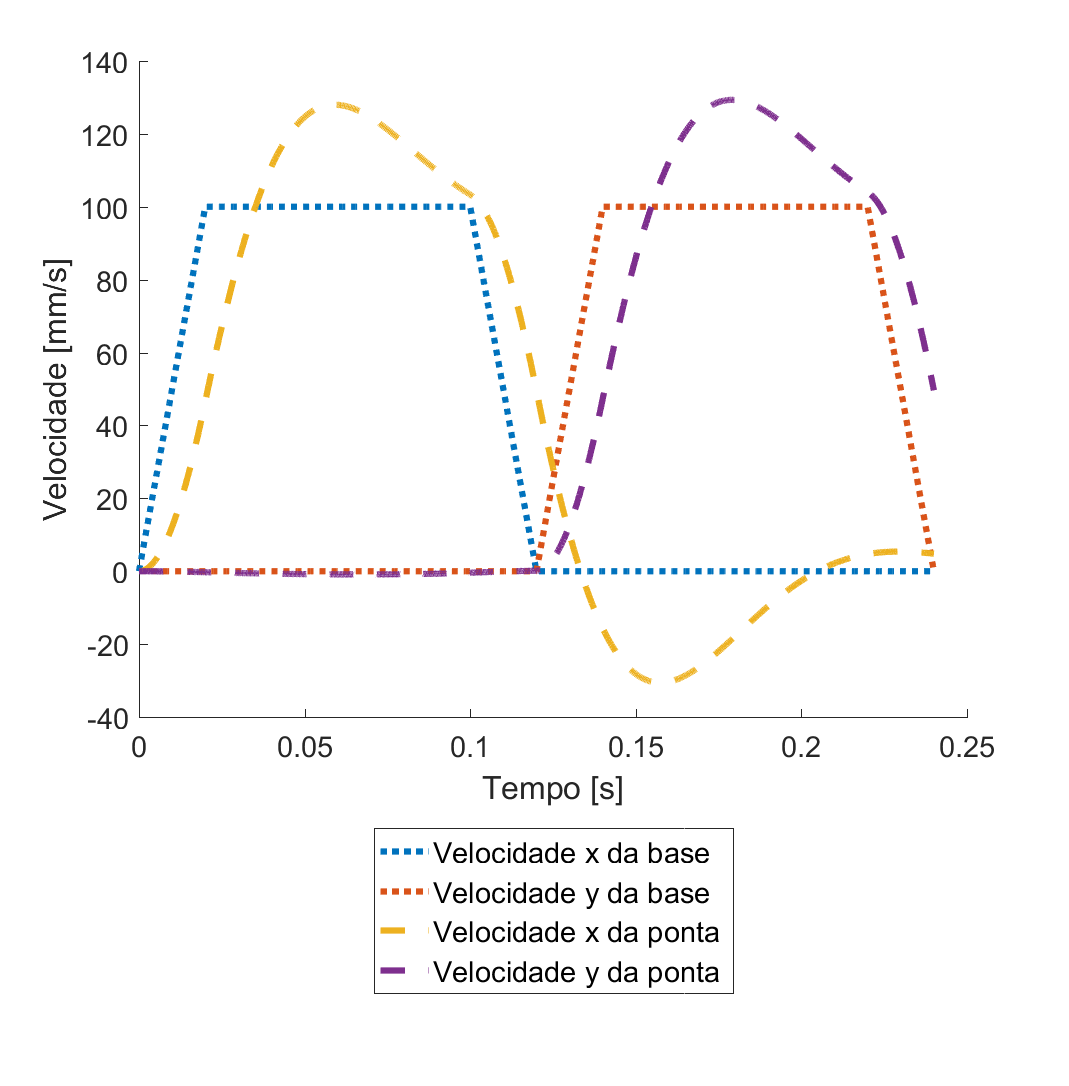
\includegraphics[width=0.38\textwidth]{Sim 1A_vel_s.png}
        \label{fig:1A_vel_s}
    }
    \hfill
    \subfigure[Com controle.]{
        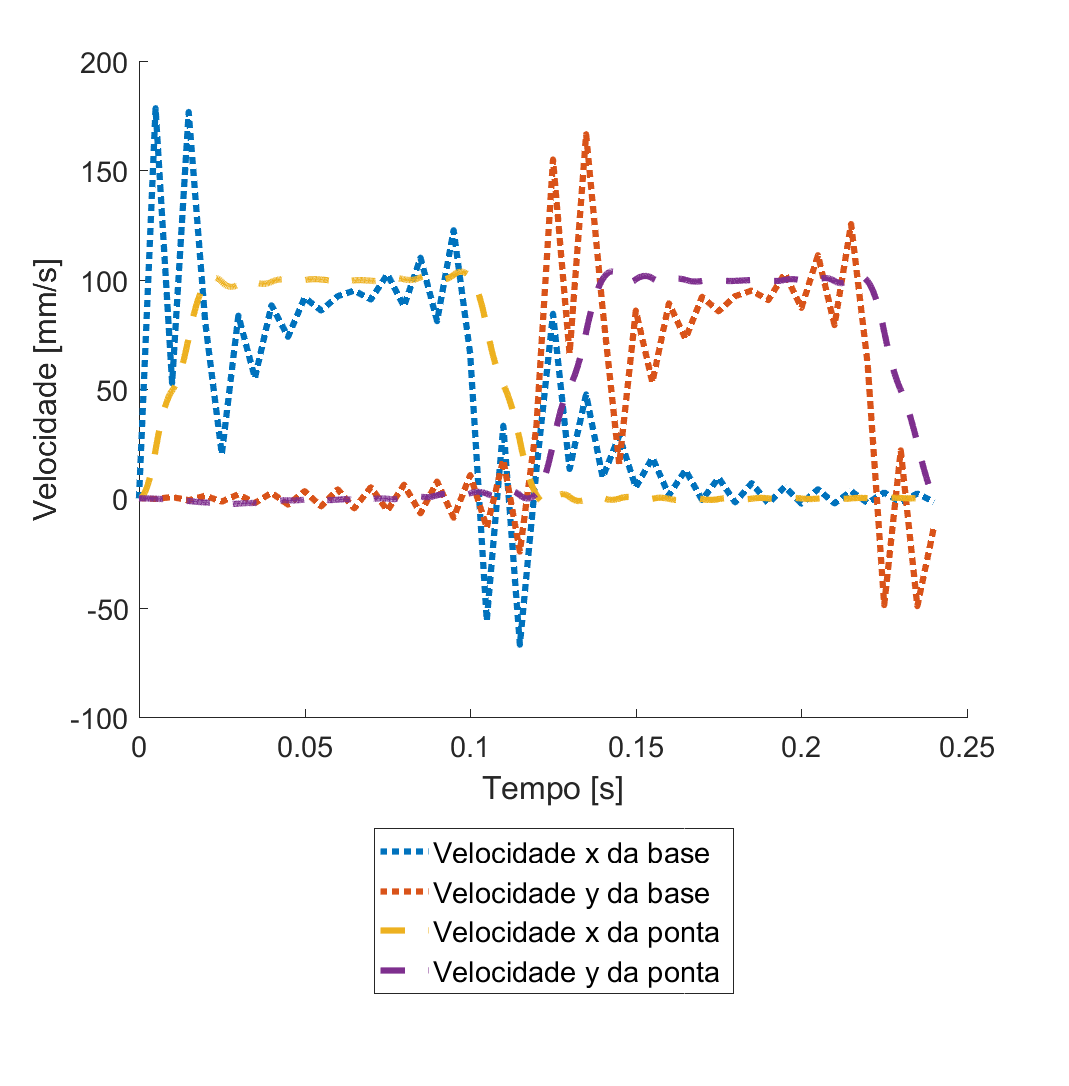
\includegraphics[width=0.38\textwidth]{Sim 1A_vel_c.png}
        \label{fig:1A_vel_c}
    }
    \label{fig:1A_vel}
  \end{figure}
\end{frame}

\begin{frame}
  \frametitle{\insertsubsection}
  \begin{figure}[H]
    \centering
    \caption{Velocidades da ponta e da base (B).}
    \subfigure[Sem controle.]{
        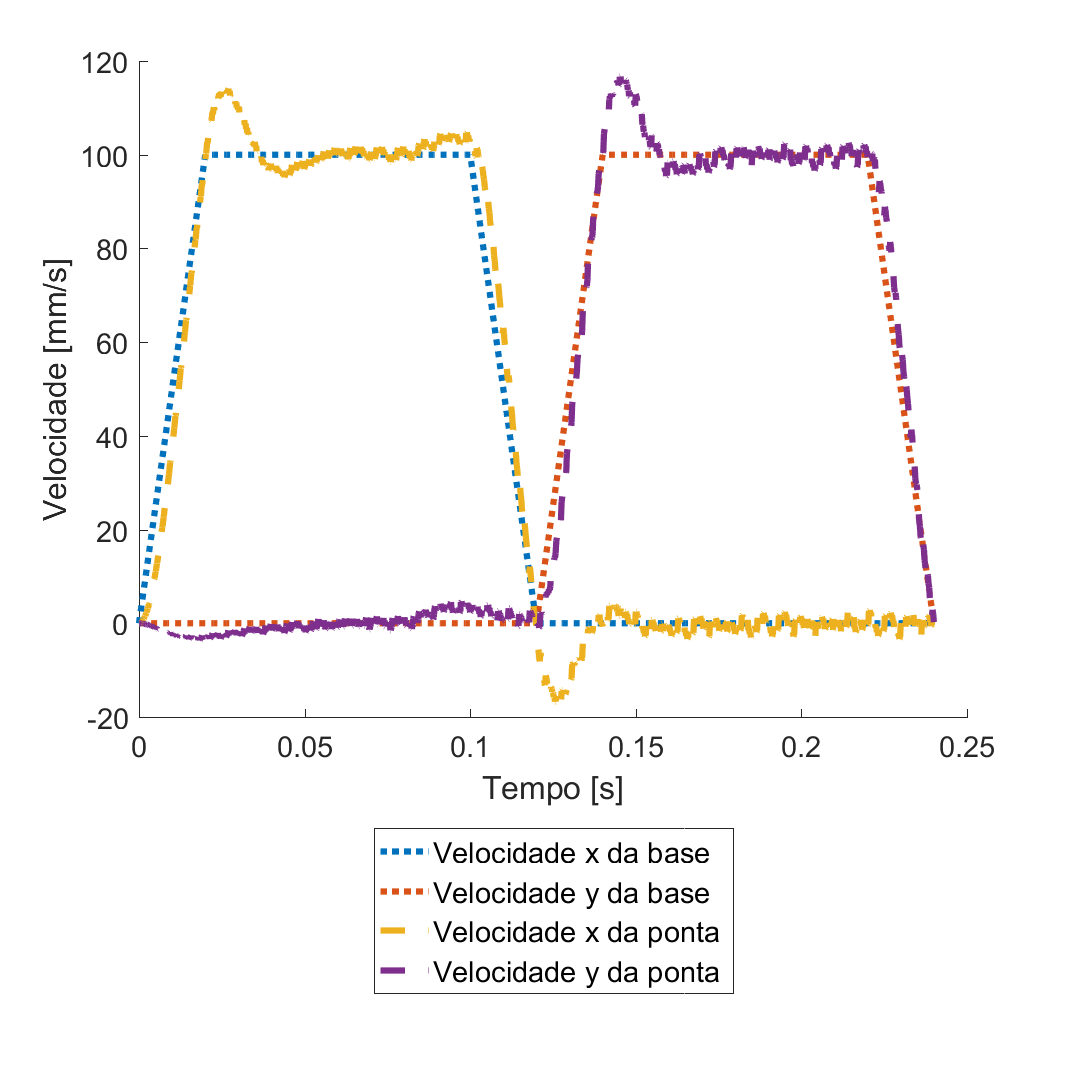
\includegraphics[width=0.38\textwidth]{Sim 1B_vel_s.png}
        \label{fig:1B_vel_s}
    }
    \hfill
    \subfigure[Com controle.]{
        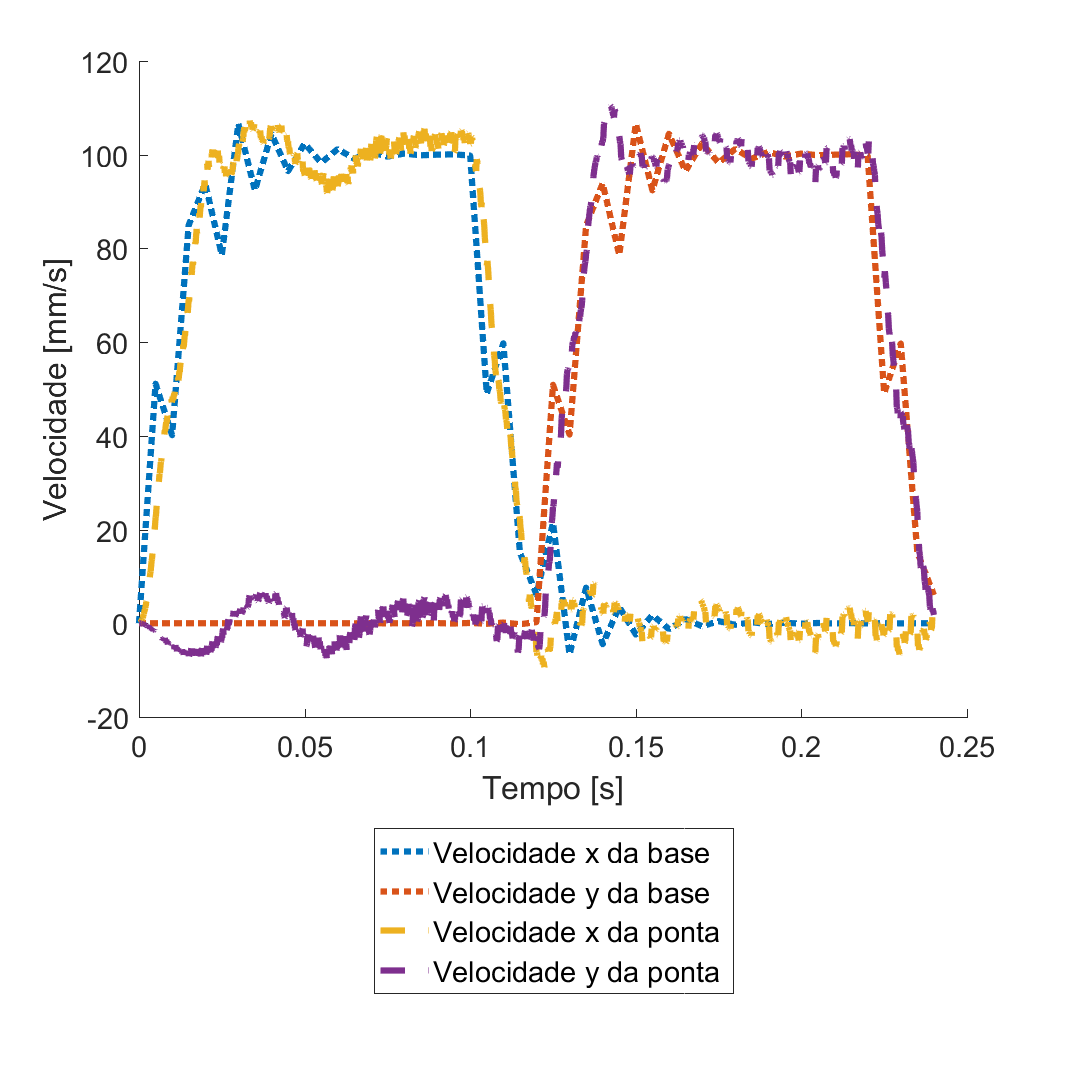
\includegraphics[width=0.38\textwidth]{Sim 1B_vel_c.png}
        \label{fig:1B_vel_c}
    }
    \label{fig:1B_vel}
  \end{figure}
\end{frame}

\subsection{\insertsectionnumber .\insertsubsectionnumber . Simulação - Variação do Coeficiente de Amortecimento (0 - 1)}

\begin{frame}
  \frametitle{\insertsubsection}
  \begin{figure}[H]
    \centering
    \caption{Caminhos da ponta e da base (A).}
    \subfigure[Sem controle.]{
        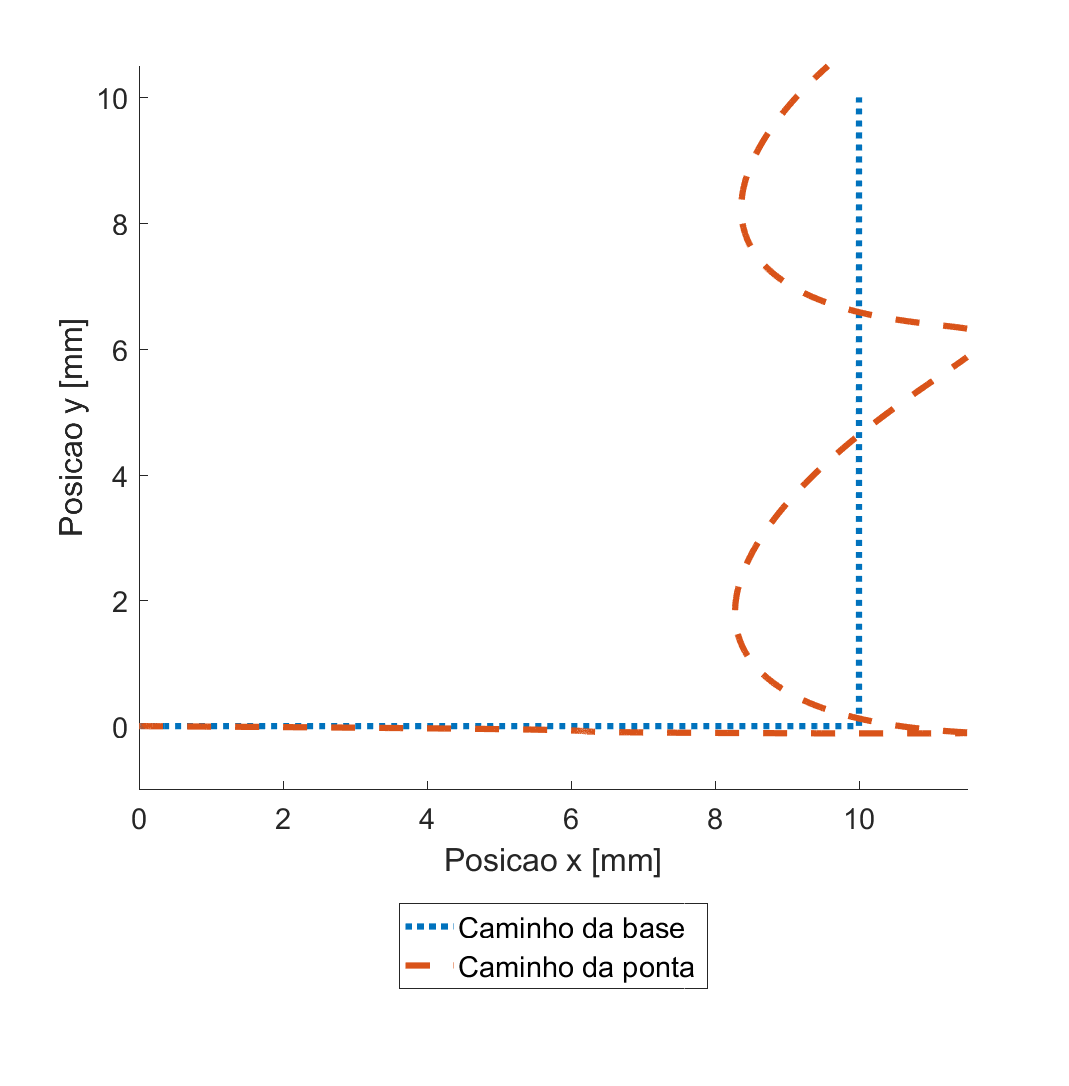
\includegraphics[width=0.38\textwidth]{Sim 2A_cam_s.png}
        \label{fig:2A_cam_s}
    }
    \hfill
    \subfigure[Com controle.]{
        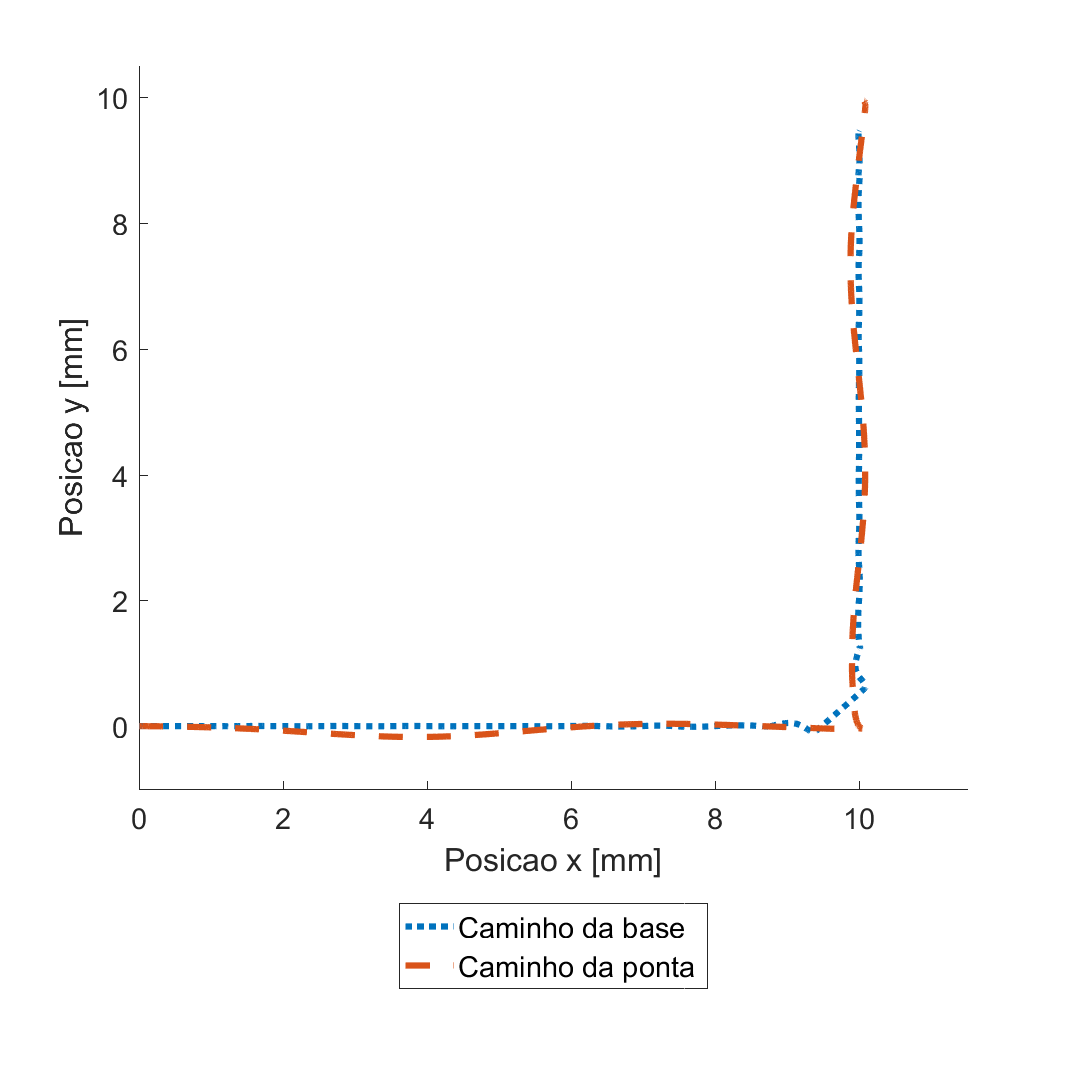
\includegraphics[width=0.38\textwidth]{Sim 2A_cam_c.png}
        \label{fig:2A_cam_c}
    }
  \end{figure}
\end{frame}

\begin{frame}
  \frametitle{\insertsubsection}
  \begin{figure}[H]
    \centering
    \caption{Caminhos da ponta e da base - Detalhamento (A)}
    \subfigure[Sem controle.]{
        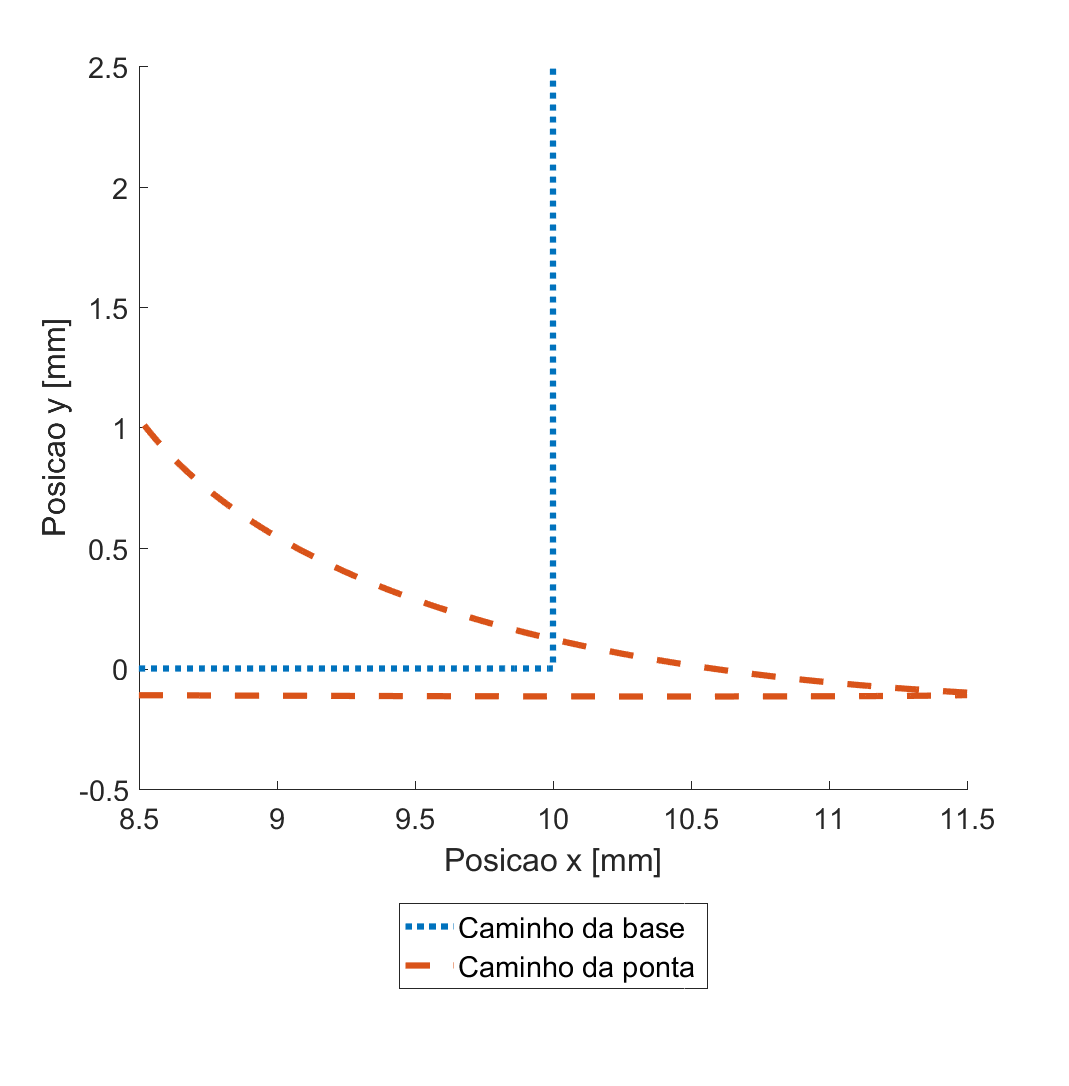
\includegraphics[width=0.38\textwidth]{Sim 2A_cam_s_zoom.png}
        \label{fig:2A_cam_s_zoom}
    }
    \hfill
    \subfigure[Com controle.]{
        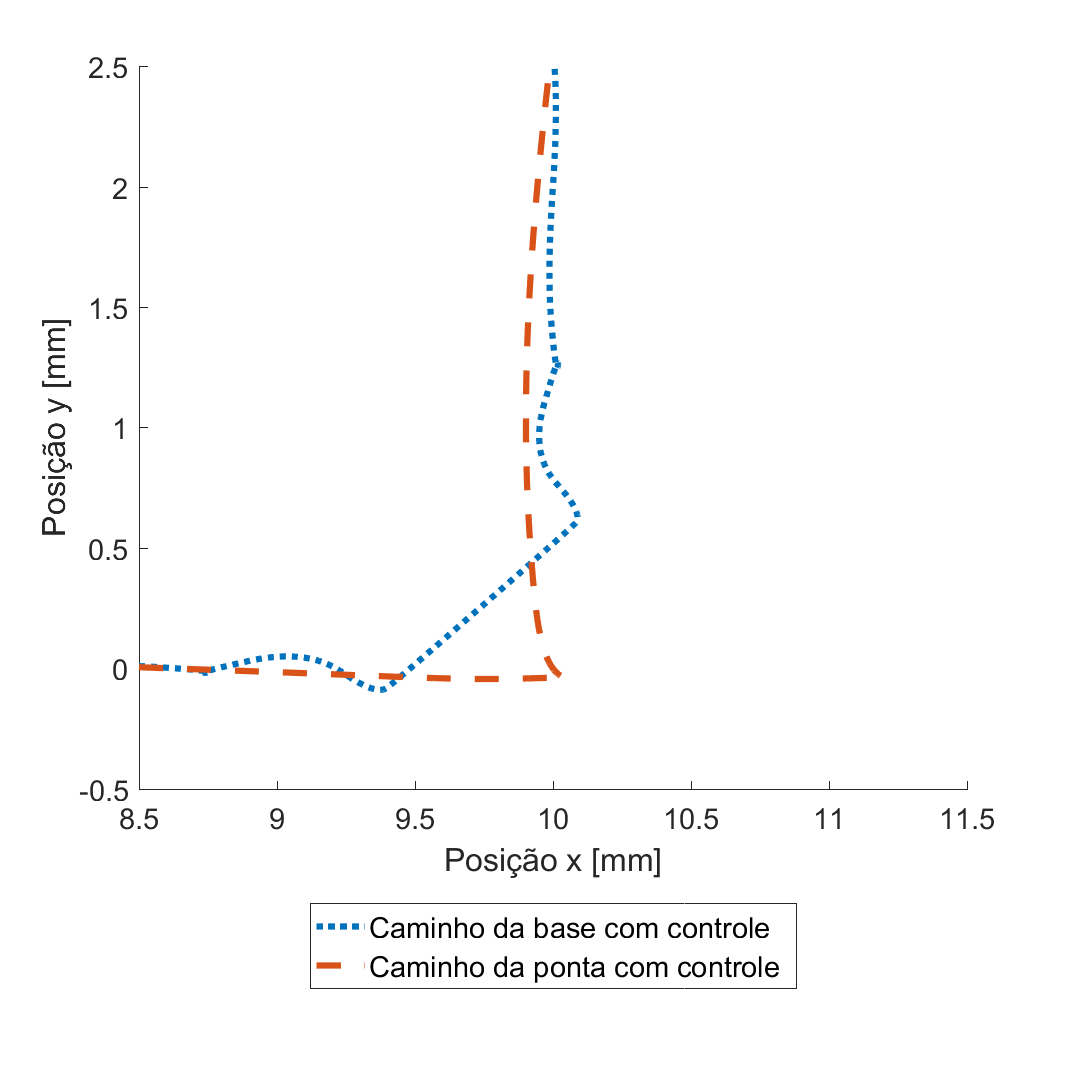
\includegraphics[width=0.38\textwidth]{Sim 2A_cam_c_zoom.png}
        \label{fig:2A_cam_c_zoom}
    }
  \end{figure}
\end{frame}

\begin{frame}
  \frametitle{\insertsubsection}
  \begin{figure}[H]
    \centering
    \caption{Caminhos da ponta e da base (B).}
    \subfigure[Sem controle.]{
        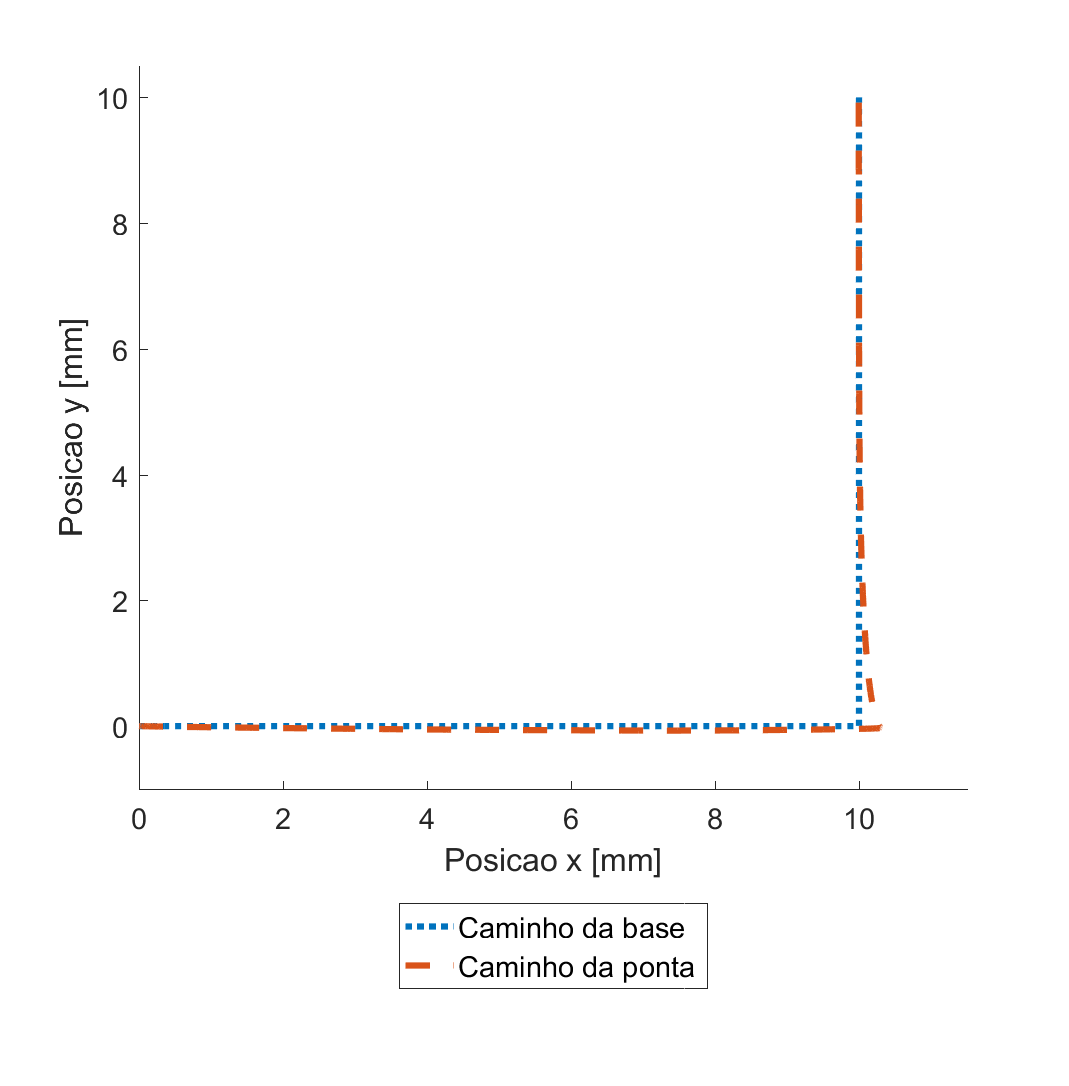
\includegraphics[width=0.38\textwidth]{Sim 2B_cam_s.png}
        \label{fig:2B_cam_s}
    }
    \hfill
    \subfigure[Com controle.]{
        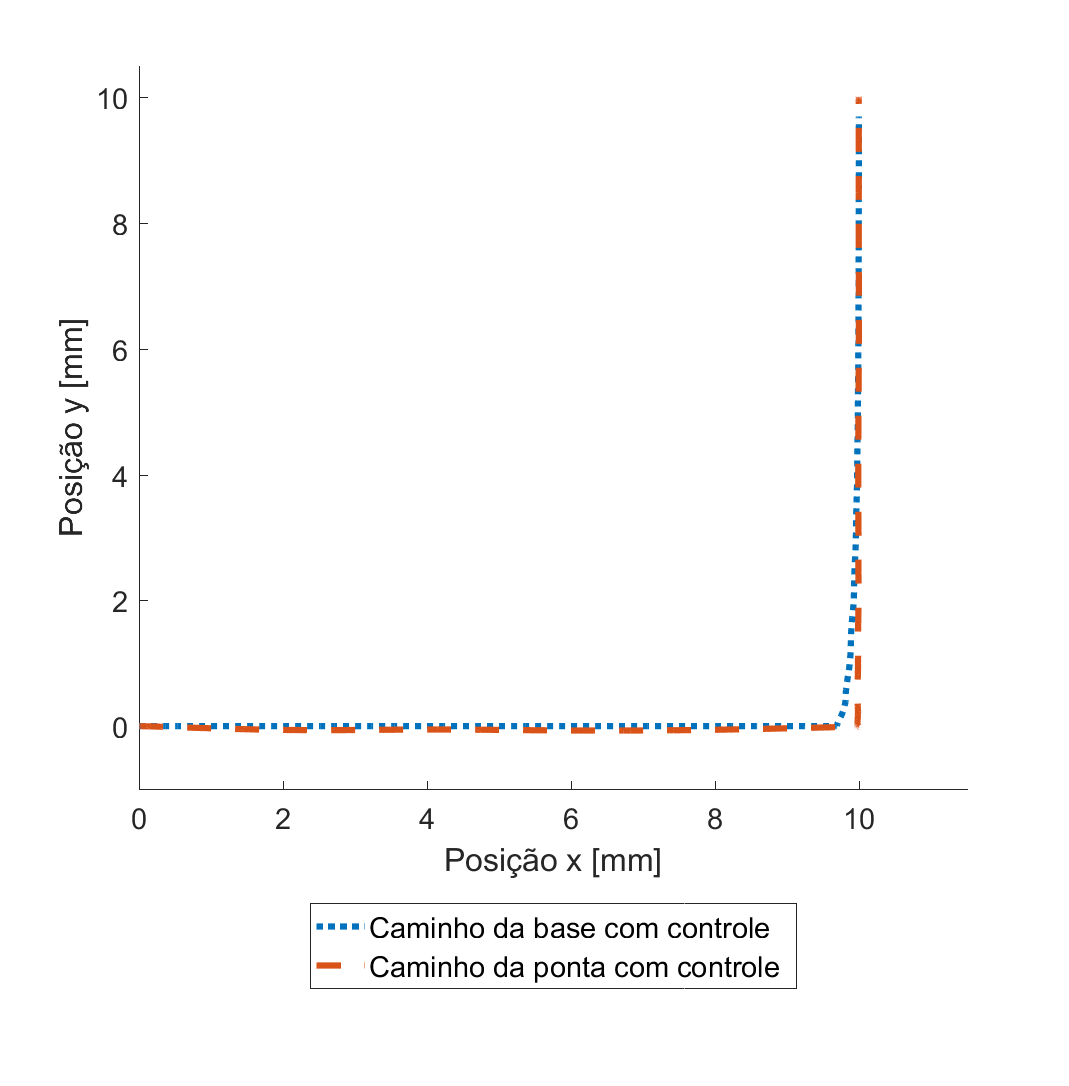
\includegraphics[width=0.38\textwidth]{Sim 2B_cam_c.png}
        \label{fig:2B_cam_c}
    }
  \end{figure}
\end{frame}

\begin{frame}
  \frametitle{\insertsubsection}
  \begin{figure}[H]
    \centering
    \caption{Caminhos da ponta e da base - Detalhamento (B)}
    \subfigure[Sem controle.]{
        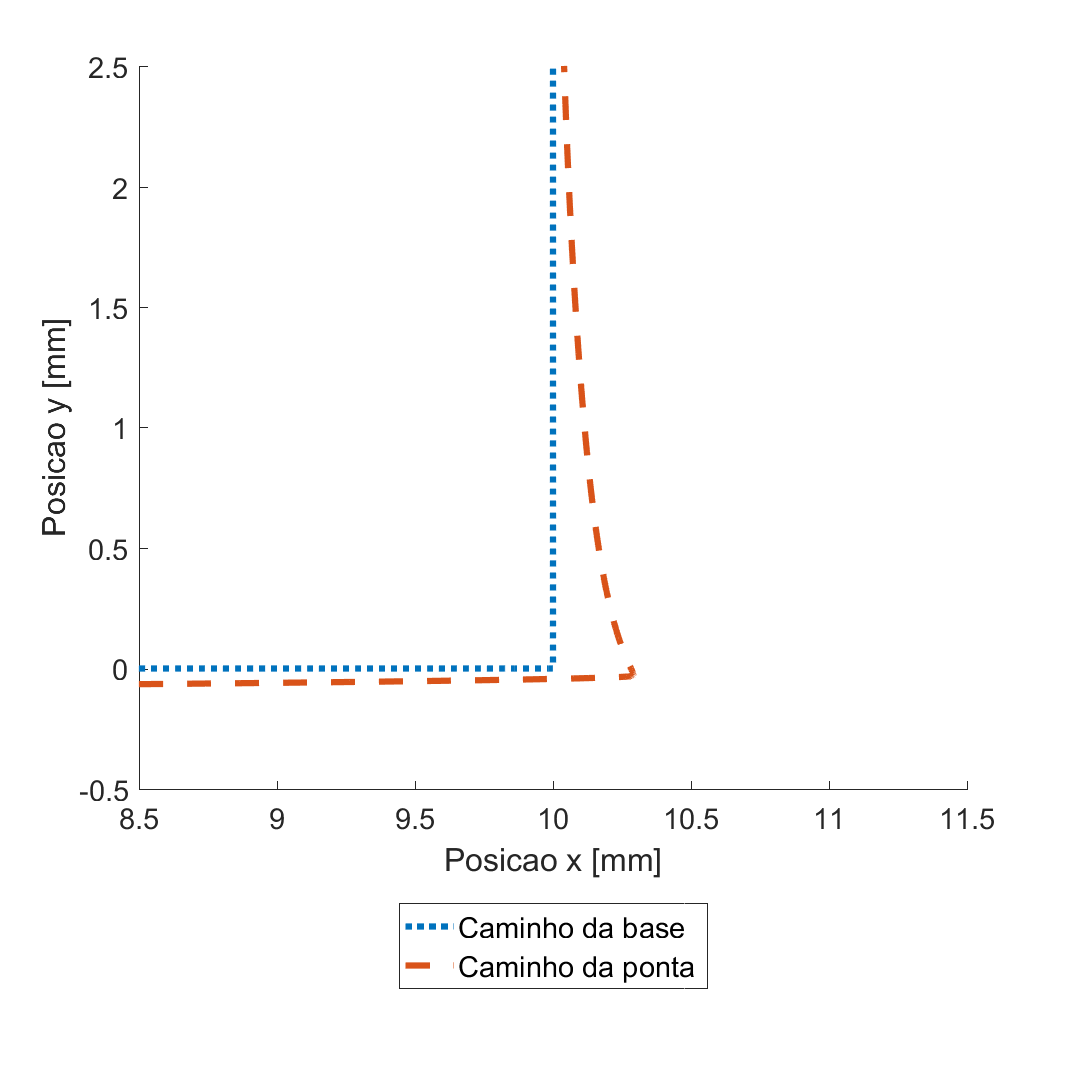
\includegraphics[width=0.38\textwidth]{Sim 2B_cam_s_zoom.png}
        \label{fig:2B_cam_s_zoom}
    }
    \hfill
    \subfigure[Com controle.]{
        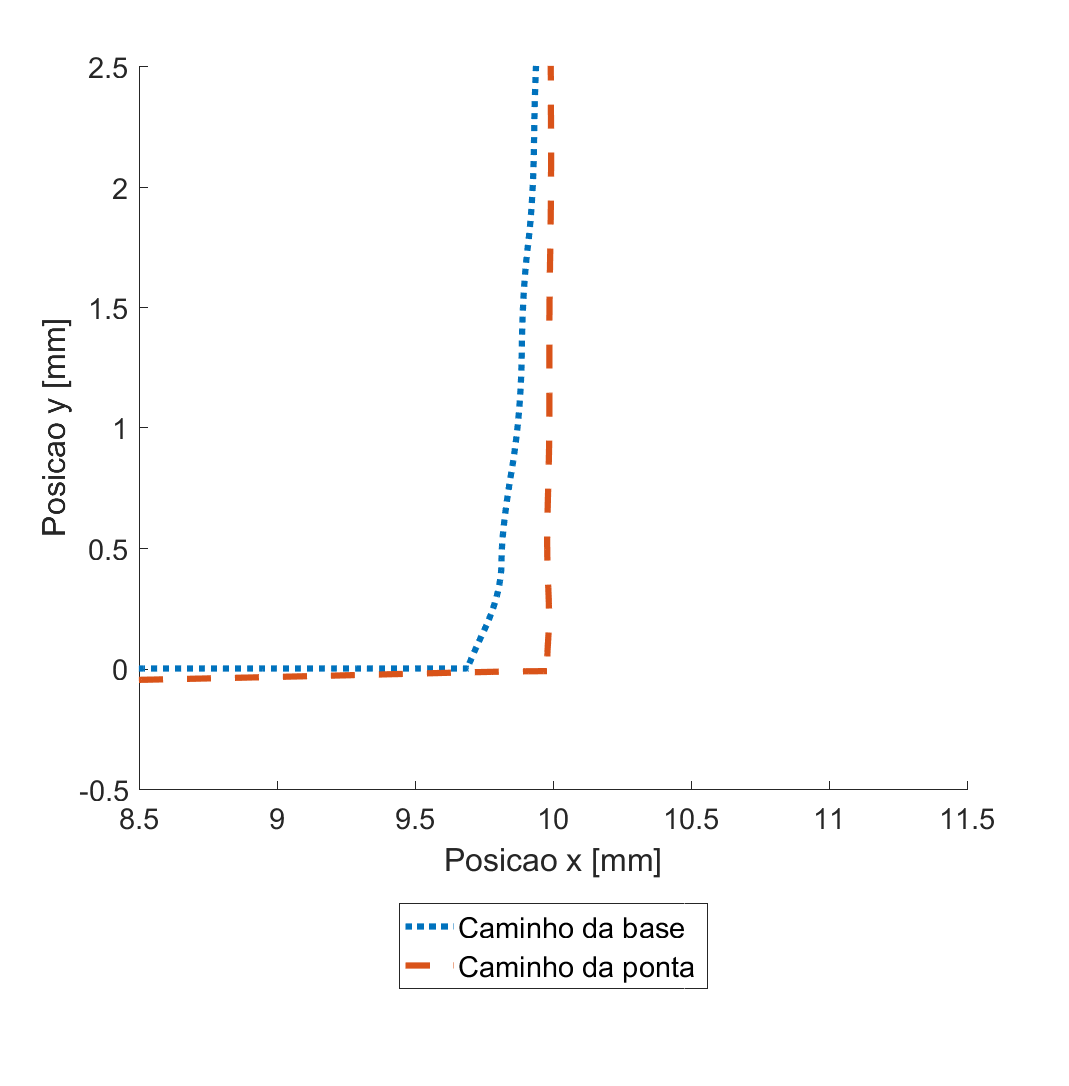
\includegraphics[width=0.38\textwidth]{Sim 2B_cam_c_zoom.png}
        \label{fig:2B_cam_c_zoom}
    }
  \end{figure}
\end{frame}

\subsection{\insertsectionnumber .\insertsubsectionnumber . Simulação - Variação na Aceleração (1000$mm/s^2$ - 10000$mm/s^2$)}

\begin{frame}
  \frametitle{\insertsubsection}
  \begin{figure}[H]
    \centering
    \caption{Caminhos da ponta e da base - Detalhamento (A)}
    \subfigure[Sem controle.]{
        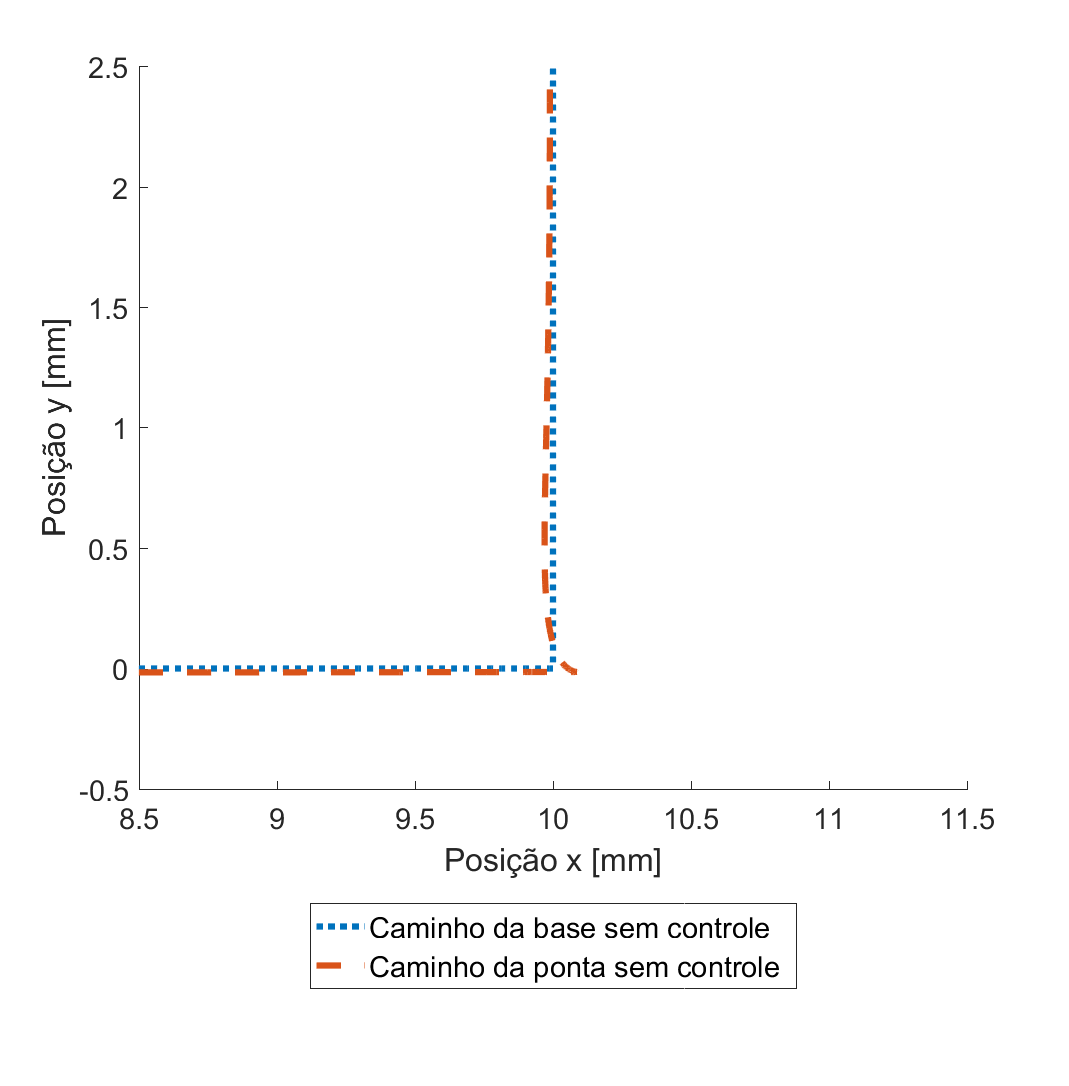
\includegraphics[width=0.38\textwidth]{Sim 3A_cam_s_zoom.png}
        \label{fig:3A_cam_s_zoom}
    }
    \hfill
    \subfigure[Com controle.]{
        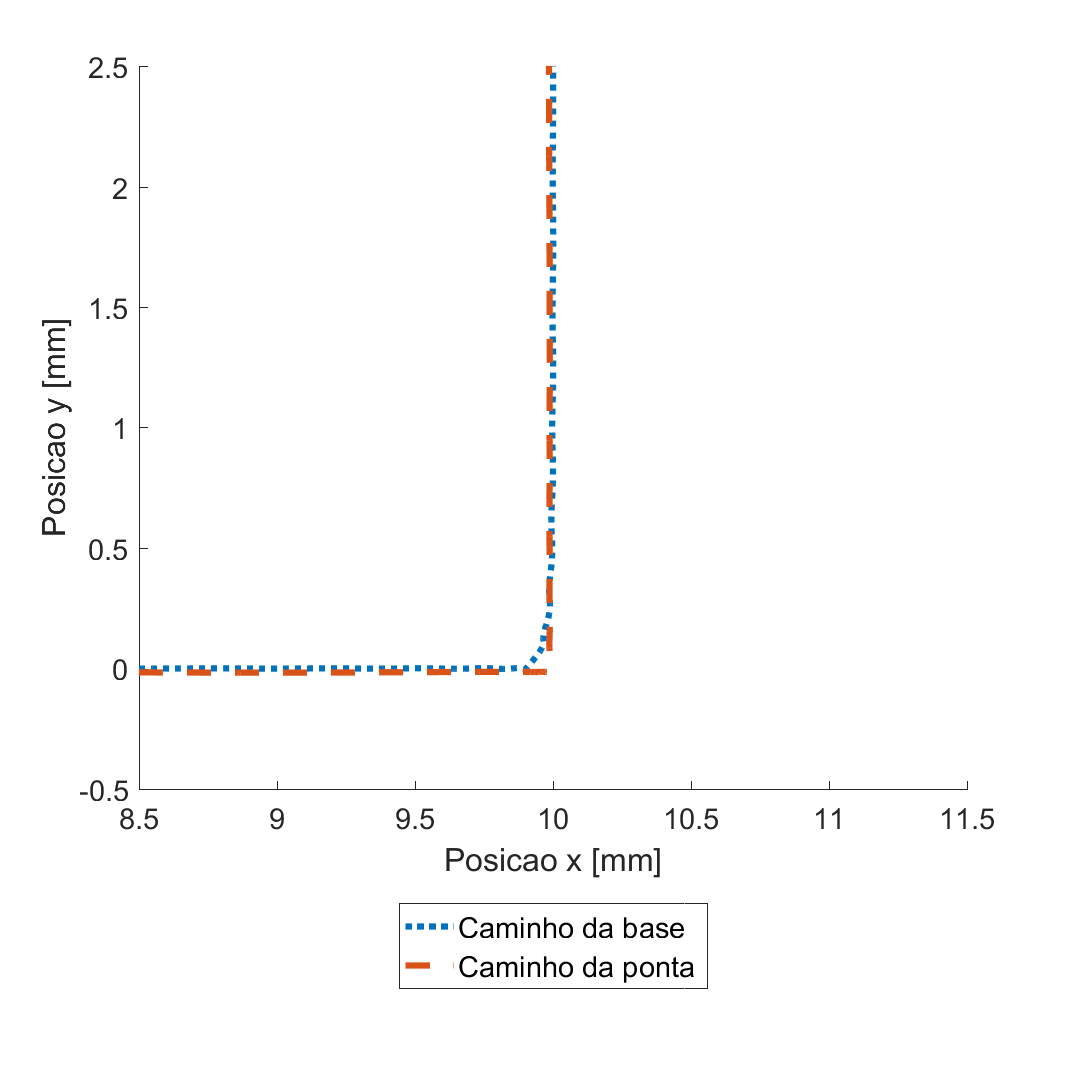
\includegraphics[width=0.38\textwidth]{Sim 3A_cam_c_zoom.png}
        \label{fig:3A_cam_c_zoom}
    }
  \end{figure}
\end{frame}

\begin{frame}
  \frametitle{\insertsubsection}
  \begin{figure}[H]
    \centering
    \caption{Caminhos da ponta e da base - Detalhamento (B)}
    \subfigure[Sem controle.]{
        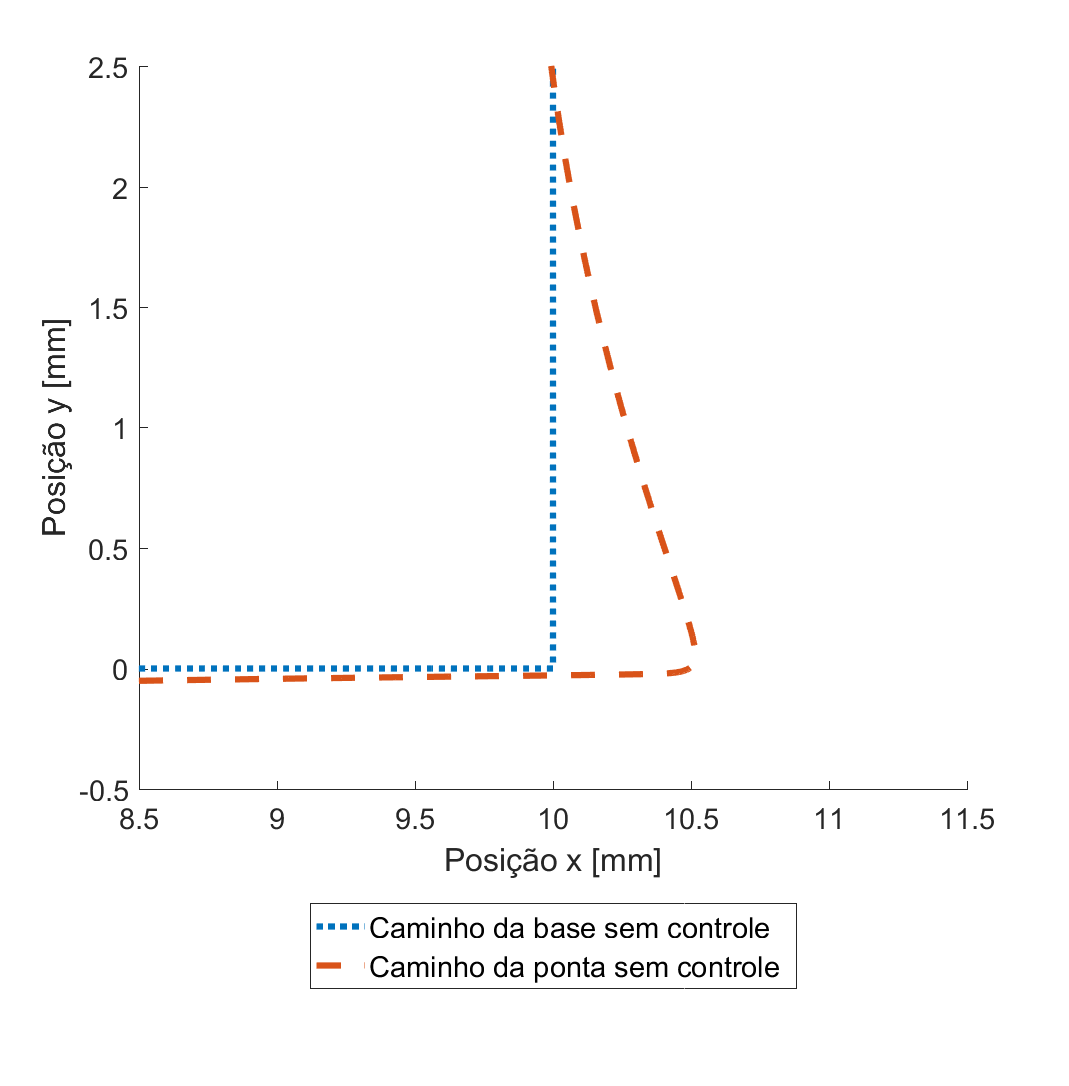
\includegraphics[width=0.38\textwidth]{Sim 3B_cam_s_zoom.png}
        \label{fig:3B_cam_s_zoom}
    }
    \hfill
    \subfigure[Com controle.]{
        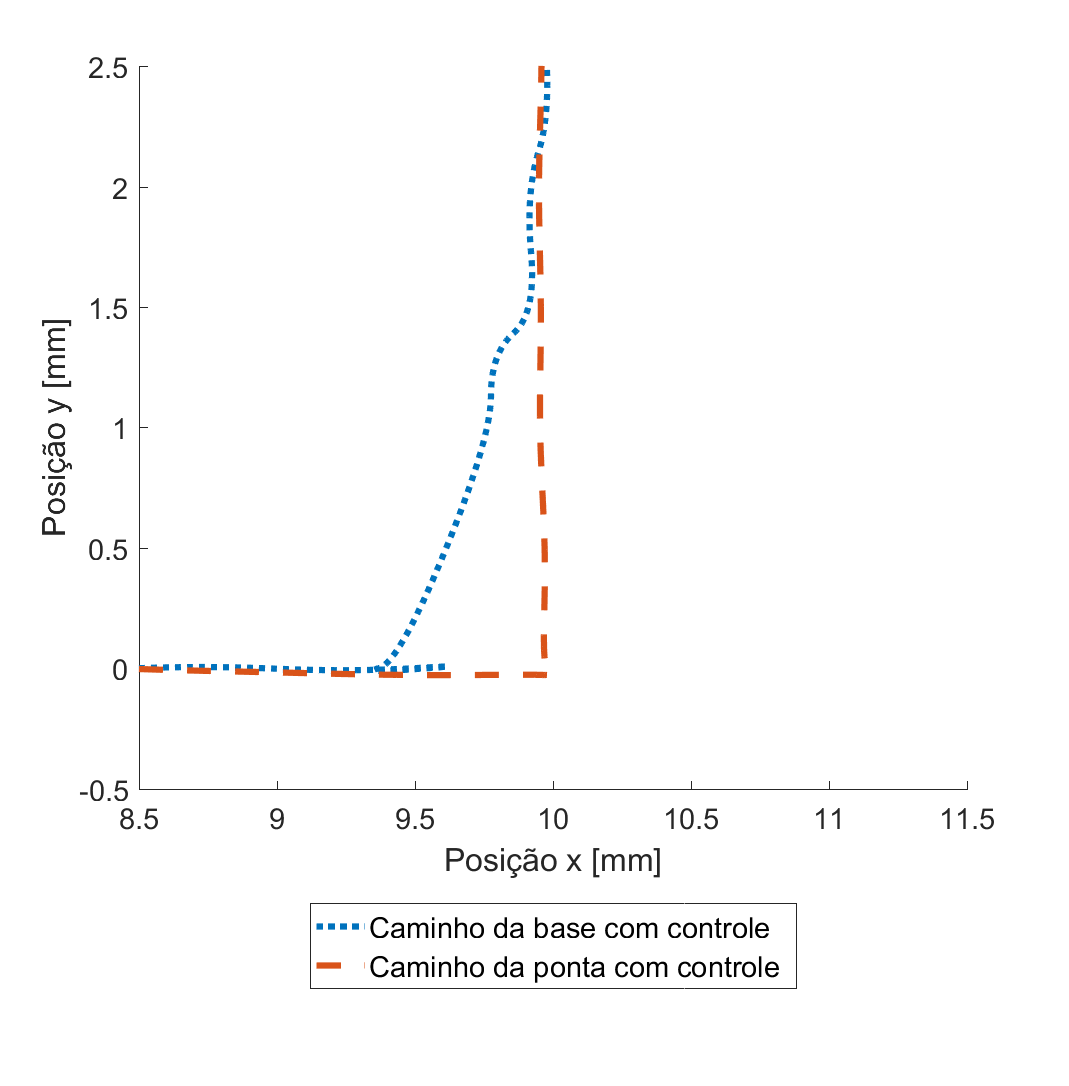
\includegraphics[width=0.38\textwidth]{Sim 3B_cam_c_zoom.png}
        \label{fig:3B_cam_c_zoom}
    }
  \end{figure}
\end{frame}

\begin{frame}
  \frametitle{\insertsubsection}
  \begin{figure}[H]
    \centering
    \caption{Velocidades da ponta e da base (A).}
    \subfigure[Sem controle.]{
        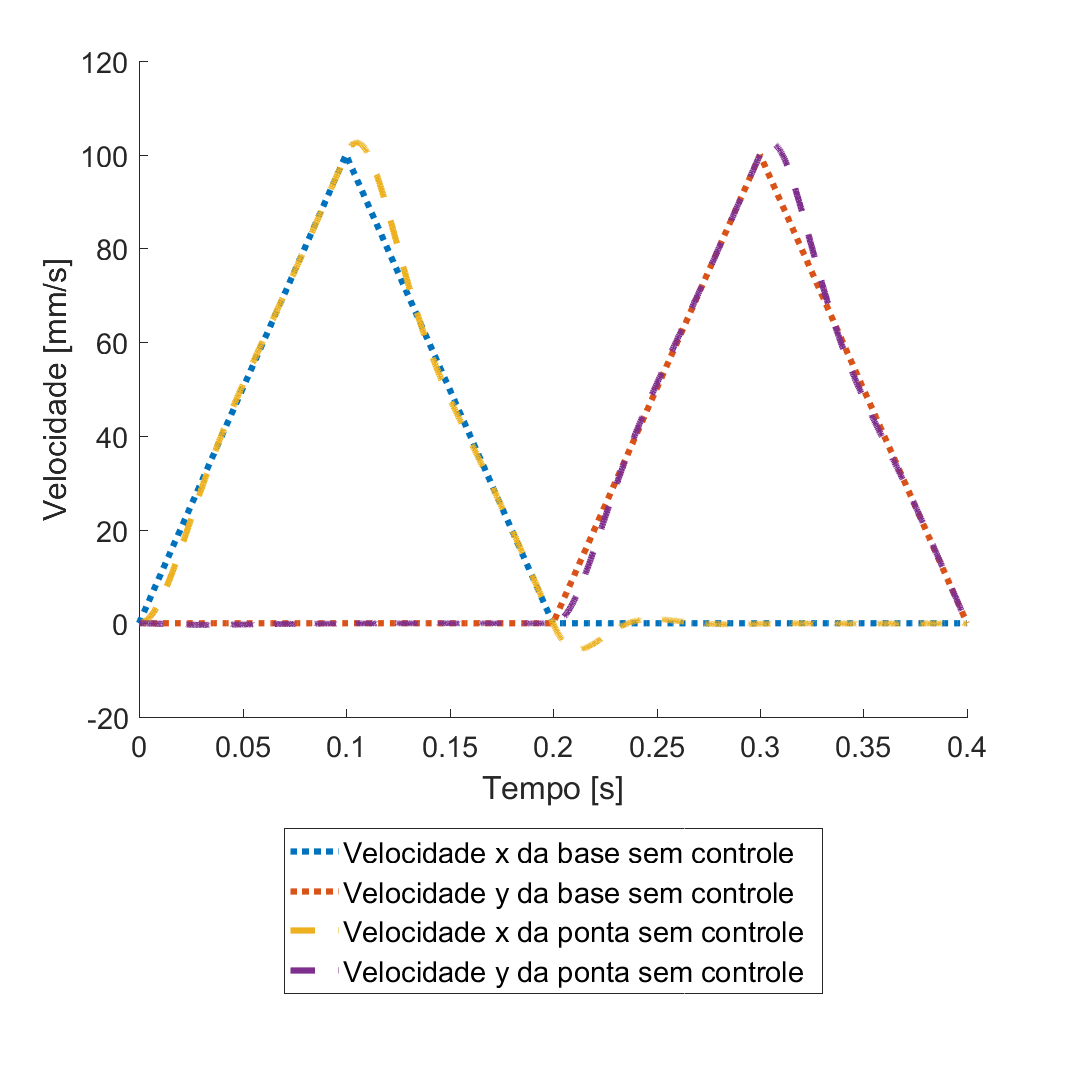
\includegraphics[width=0.38\textwidth]{Sim 3A_vel_s.png}
        \label{fig:3A_vel_s}
    }
    \hfill
    \subfigure[Com controle.]{
        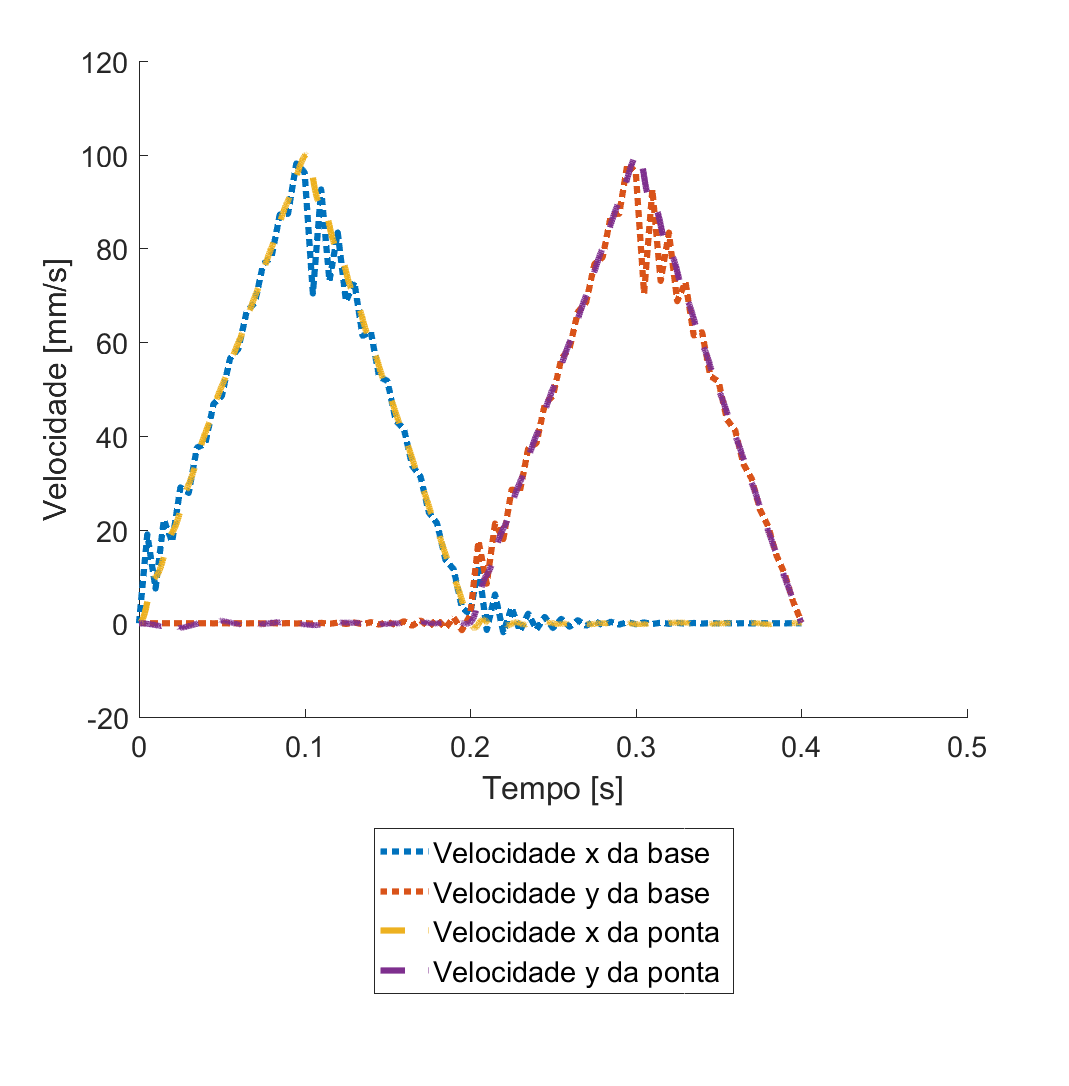
\includegraphics[width=0.38\textwidth]{Sim 3A_vel_c.png}
        \label{fig:3A_vel_c}
    }
    \label{fig:3A_vel}
  \end{figure}
\end{frame}

\begin{frame}
  \frametitle{\insertsubsection}
  \begin{figure}[H]
    \centering
    \caption{Velocidades da ponta e da base (B).}
    \subfigure[Sem controle.]{
        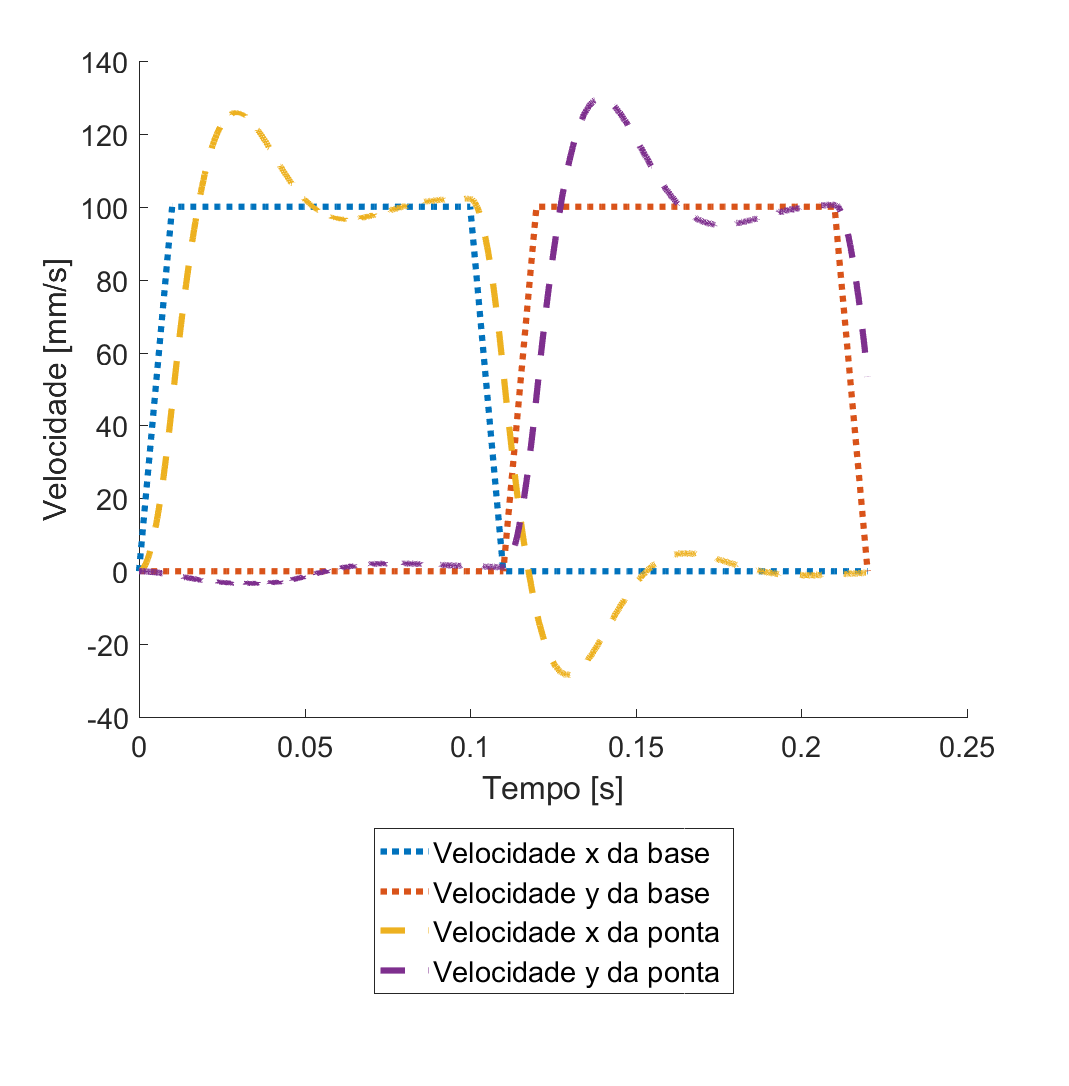
\includegraphics[width=0.38\textwidth]{Sim 3B_vel_s.png}
        \label{fig:3B_vel_s}
    }
    \hfill
    \subfigure[Com controle.]{
        \includegraphics[width=0.38\textwidth]{Sim 3B_vel_c.png}
        \label{fig:3B_vel_c}
    }
    \label{fig:3B_vel}
  \end{figure}
\end{frame}

\subsection{\insertsectionnumber .\insertsubsectionnumber . Simulação - Variação da Velocidade desejada (50$mm/s$ - 200$mm/s$)}

\begin{frame}
  \frametitle{\insertsubsection}
  \begin{figure}[H]
    \centering
    \caption{Caminhos da ponta e da base - Detalhamento (A)}
    \subfigure[Sem controle.]{
        \includegraphics[width=0.38\textwidth]{Sim 5A_cam_s_zoom.png}
        \label{fig:5A_cam_s_zoom}
    }
    \hfill
    \subfigure[Com controle.]{
        \includegraphics[width=0.38\textwidth]{Sim 5A_cam_c_zoom.png}
        \label{fig:5A_cam_c_zoom}
    }
  \end{figure}
\end{frame}

\begin{frame}
  \frametitle{\insertsubsection}
  \begin{figure}[H]
    \centering
    \caption{Caminhos da ponta e da base - Detalhamento (B)}
    \subfigure[Sem controle.]{
        \includegraphics[width=0.38\textwidth]{Sim 5B_cam_s_zoom.png}
        \label{fig:5B_cam_s_zoom}
    }
    \hfill
    \subfigure[Com controle.]{
        \includegraphics[width=0.38\textwidth]{Sim 5B_cam_c_zoom.png}
        \label{fig:5B_cam_c_zoom}
    }
  \end{figure}
\end{frame}

\begin{frame}
  \frametitle{\insertsubsection}
  \begin{figure}[H]
    \centering
    \caption{Velocidades da ponta e da base (A).}
    \subfigure[Sem controle.]{
        \includegraphics[width=0.38\textwidth]{Sim 5A_vel_s.png}
        \label{fig:5A_vel_s}
    }
    \hfill
    \subfigure[Com controle.]{
        \includegraphics[width=0.38\textwidth]{Sim 5A_vel_c.png}
        \label{fig:5A_vel_c}
    }
    \label{fig:5A_vel}
  \end{figure}
\end{frame}

\begin{frame}
  \frametitle{\insertsubsection}
  \begin{figure}[H]
    \centering
    \caption{Velocidades da ponta e da base (B).}
    \subfigure[Sem controle.]{
        \includegraphics[width=0.38\textwidth]{Sim 5B_vel_s.png}
        \label{fig:5B_vel_s}
    }
    \hfill
    \subfigure[Com controle.]{
        \includegraphics[width=0.38\textwidth]{Sim 5B_vel_c.png}
        \label{fig:5B_vel_c}
    }
    \label{fig:5B_vel}
  \end{figure}
\end{frame}

\subsection{\insertsectionnumber .\insertsubsectionnumber . Simulação - Variação do Passo de tempo (0,1$s$ - 0,001$s$)}

\begin{frame}
  \frametitle{\insertsubsection}
  \begin{figure}[H]
    \centering
    \caption{Caminhos da ponta e da base - Detalhamento (A)}
    \subfigure[Sem controle.]{
        \includegraphics[width=0.38\textwidth]{Sim 4A_cam_s_zoom.png}
        \label{fig:4A_cam_s_zoom}
    }
    \hfill
    \subfigure[Com controle.]{
        \includegraphics[width=0.38\textwidth]{Sim 4A_cam_c_zoom.png}
        \label{fig:4A_cam_c_zoom}
    }
  \end{figure}
\end{frame}

\begin{frame}
  \frametitle{\insertsubsection}
  \begin{figure}[H]
    \centering
    \caption{Caminhos da ponta e da base - Detalhamento (B)}
    \subfigure[Sem controle.]{
        \includegraphics[width=0.38\textwidth]{Sim 4B_cam_s_zoom.png}
        \label{fig:4B_cam_s_zoom}
    }
    \hfill
    \subfigure[Com controle.]{
        \includegraphics[width=0.38\textwidth]{Sim 4B_cam_c_zoom.png}
        \label{fig:4B_cam_c_zoom}
    }
  \end{figure}
\end{frame}

\begin{frame}
  \frametitle{\insertsubsection}
  \begin{figure}[H]
    \centering
    \caption{Velocidades da ponta e da base (A).}
    \subfigure[Sem controle.]{
        \includegraphics[width=0.38\textwidth]{Sim 4A_vel_s.png}
        \label{fig:4A_vel_s}
    }
    \hfill
    \subfigure[Com controle.]{
        \includegraphics[width=0.38\textwidth]{Sim 4A_vel_c.png}
        \label{fig:4A_vel_c}
    }
    \label{fig:4A_vel}
  \end{figure}
\end{frame}

\begin{frame}
  \frametitle{\insertsubsection}
  \begin{figure}[H]
    \centering
    \caption{Velocidades da ponta e da base (B).}
    \subfigure[Sem controle.]{
        \includegraphics[width=0.38\textwidth]{Sim 4B_vel_s.png}
        \label{fig:4B_vel_s}
    }
    \hfill
    \subfigure[Com controle.]{
        \includegraphics[width=0.38\textwidth]{Sim 4B_vel_c.png}
        \label{fig:4B_vel_c}
    }
    \label{fig:4B_vel}
  \end{figure}
\end{frame}

\section{\insertsectionnumber . Conclusão}

\begin{frame}
  \frametitle{\insertsection}
  \begin{itemize}
    \item A implementação do método demonstrou uma diminuição notável no desvio do caminho da ponta quando comparado ao caminho simulado sem controle de trajetória.
    \item Os resultados obtidos por meio de simulações confirmaram a capacidade do controle em atenuar as complexidades dinâmicas do sistema.
    \item Uma possível melhoria é a utilização de diferentes passos de tempo para reduzir a carga computacional, através de chutes iniciais melhores. 
  \end{itemize}
\end{frame}

% Remove a logo para o próximo slide
\setbeamertemplate{logo}{}
\begin{frame}
    
  \backgroundlogo
  \begin{center}
    \huge{Obrigado!}
  \end{center}
\end{frame}

\bibliographystyle{abntex2-alf}      
\bibliography{referencias}	

\end{document}